%!TEX root = ../thesis.tex
%*******************************************************************************
%****************************** Third Chapter *********************************
%*******************************************************************************

% \chapter{Mean level eQTL mapping using single cell RNA-seq data from iPSCs}
\chapter{Comparison of eQTL mapping using bulk and single cell RNA-seq readouts}
\label{chapter3}

% abstract
As discussed in \textbf{section 
\ref{sec:eqtl}},
% 1.1.8}, 
in traditional 
eQTL
% \gls{eqtl}
mapping 
individual-level 
gene expression 
% profiles are 
is
measured using bulk RNA-sequencing, where 
the quantified 
% gene 
expression profiles represent
% expression level is averaged across 
several thousands of cells from each individual.
As we have seen, recent technological advances 
% in experimental techniques 
have allowed molecular phenotypes, including gene expression, to be assayed at the level of single cells.
In particular, 
scRNA-seq
% \gls{scrnaseq} 
% assays are now well established,
is now an established technique, 
and can be deployed at population-scale, across several individuals.
% and computational methods to analyse the data have become fairly standardised.
% with fairly standardised methods for performing both low-level analyses and complex tasks, such as clustering and pseudotime estimation.
Owing to their ability to identify cell types and cell states in a data-driven manner,
% no references in abstract?
% \cite{buettner2015computational},
% \gls{scrnaseq} 
scRNA-seq
data from a single experiment can be used to define homogeneous cell populations, quantify expression levels within them, and then map eQTL in each of them separately.
% - and then quantify expression levels within -  the use of \gls{scrnaseq} data, 
% combined with genotype information, 
% These types of analyses can improve
% % is uniquely positioned to provide an extra layer to 
% our understanding of the genetic regulation of expression, across
% % a plethora of 
% cell types and states.
As a consequence, studies where single cell expression profiles (rather than bulk) are used to perform
% \gls{eqtl}
eQTL
mapping 
% (where the effect of common genetic variants on expression is assessed at single cell resolution)
% \gls{scrnaseq} profiles are combined with genotype information to map \gls{eqtl})
% is quickly emerging as a field of research, 
have emerged recently, and promise
% and it promises 
to greatly improve our understanding of the genetic architecture of 
gene regulation
% human disease 
across tissues, in both human disease and development.
% However, the extent to which \gls{eqtl} identified using scRNA-seq data can replicate those obtained using the `gold standard' bulk RNA-seq approach has not been explored.
% However, there has not been a systematic comparison between single cell and bulk RNA-seq obtained eQTL maps to date.
However, the use of single-cell RNA-seq to map eQTL maps as opposed to using bulk RNA-seq profiling has not been systematically benchmarked.
% However, the relationship between eQTL maps obtained using single cell data as compared to bulk data has not been systematically explored.
To address this, here
% Here,
I select a very homogeneous cell type (iPSCs), where direct comparison is possible.
In particular,
% Here, 
I use matched bulk and single cell RNA-seq from over 100 human 
% \gls{ipsc} 
iPSC lines 
% donors
to assess our ability to detect 
% \gls{eqtl} 
eQTL
using single cell RNA-seq data, and the extent to which we can replicate 
% \gls{eqtl}
eQTL
identified using bulk RNA-seq, when mapping eQTL using a common analytical framework based on LMMs (see \textbf{Chapter 
% 2
\ref{chapter2}}).
% Direct comparison is possible in this system, given the very homogeneous cell type (iPSCs).
Additionally, for a subset of lines, I compare results using two different scRNA-seq technologies.
As more and more single cell-eQTL
% \gls{eqtl}
(sc-eQTL) studies emerge, I believe that
the insights presented here will help
% this is a useful step towards 
establishing a `best practice' workflow, to optimise yield of sc-eQTL
% \gls{eqtl}
maps and to establish uniform methods across the field.
% I show preliminary results where
% we systematically assess the role played by multiple factors including the chosen aggregation method and covariates used and compare results across technologies.
% We believe this is a useful resource for several future studies that will want to perform \gls{eqtl} mapping using single cell expression profiles.

\newpage

\begin{Comment2}
% \subsection{Contributions}
\hspace{-3mm}\textbf{Contributions} 
In this chapter, I present results from two main bodies of work.

First, I describe a set of results from analyses I have conducted in the context of a larger collaborative project between the Stegle, Marioni and Vallier labs. 
In particular, the data was generated by Ludovic Vallier’s lab at the Sanger Institute, and the experiments were led by Mariya Chhatriwala, using cell lines from the \gls{hipsci} project.
Davis McCarthy and I processed the scRNA-seq data and performed quality control.
Marc Jan Bonder processed the bulk RNA-seq data.
I performed all analyses presented in the first part of this chapter, under the supervision of Oliver Stegle and John Marioni.
% The text from which this chapter is based was written collaboratively by myself, John Marioni and Oliver Stegle.
The code for processing, analysing and plotting the data is open source and freely accessible here: \url{https://github.com/single-cell-genetics/singlecell\_endodiff\_paper}.\
The paper 
% \cite{cuomo2020single}
is available at \url{https://www.nature.com/articles/s41467-020-14457-z} and has been published as:\\

Anna S.E. Cuomo*, Daniel D. Seaton*, Davis J. McCarthy*, Iker Martinez, Marc Jan Bonder, Jose Garcia-Bernardo, Shradha Amatya, Pedro Madrigal, Abigail Isaacson, Florian Buettner, Andrew Knights, Kedar Nath Natarajan, the Hipsci Consortium, Ludovic Vallier, John C. Marioni, Mariya Chhatriwala, Oliver Stegle. Single-cell RNA-sequencing of differentiating iPS cells reveals dynamic genetic effects on gene expression. \textit{Nature Communications}, 2020, (* equal contribution)\\


In the second part of this chapter, I present more recent preliminary results from work in collaboration with Giordano Alvari and Marc Jan Bonder, from the Stegle lab.
This project was designed by Marc Jan Bonder and myself, to extend the results presented in the first part of this chapter.
Giordano performed most of the analyses, under mine and Marc Jan Bonder's supervision.
Marc Jan Bonder and I performed the remaining analyses and summarised the results.\\

I generated all figures included in this chapter, except where indicated otherwise in figure legends.
% between the Stegle, Bonder and McCarthy labs.
% The project was lead by Giordano Alvari under Marc Jan Bonder's supervision and mine.
% Christina Azodi supervised by Davis McCarthy performed the simulation analyses.
% \vfill
\end{Comment2}

\newpage

\section{Introduction}

As outlined in \textbf{section 
% 1.1.8},
\ref{sec:eqtl}} 
since the publication of the first human \gls{eqtl} map in 2003 \cite{schadt2003genetics}, the field has adapted to adopt technological advances as they emerged, both in terms of statistical approaches (from linkage analysis to genome-wide scans), and of new technologies for the estimation of gene expression (from microarrays to RNA-seq).
I use this section to give a brief overview of methods to estimate gene expression (\textbf{section \ref{sec:gene_expression}}), the advent of single cell RNA-seq (\textbf{section \ref{sec:scrnaseq}}) and the consequent birth of the (very new) single cell-\gls{eqtl} mapping field of research (\textbf{section \ref{sec:sc_eqtl}}). 

\subsection{Measuring gene expression}
\label{sec:gene_expression}

Early methods for estimating the number of expressed mRNA molecules associated with a particular gene (hereafter defined as a gene's expression)
% to estimate the RNA levels of genes 
were Northern blots \cite{alwine1977method} and quantitative reverse transcription polymerase chain reaction, qRT-PCR \cite{gibson1996novel}. 
In Northern blots, electrophoresis is used to separate RNA, which is then visualised by hybridisation with labelled probes. 
A key limitation of Northern blots is that they require large amounts of input material and the results are mostly only qualitative.
% , at most semi-quantitative.
In qRT-PCR, RNA is reverse-transcribed into complementary DNA (cDNA) and then amplified using PCR, after each cycle of which the concentration of DNA is measured using a fluorescent dye. 
This required normalisation relative to a standard gene (e.g. 
housekeeping genes, or 
ribosomal genes) which was assumed to be `stable', making this method also not very quantitative.
% both are low-throughput
Additionally, both of these methods were very low-throughput, typically used only to quantify one, or at most few genes - hence being referred to as `single gene approaches'.
% Additionally, these methods were not very accurate, as the quantification of each gene required normalisation relative to a standard gene
% of known sequence and quantity, called an RNA spike-in.
% \footnote{An RNA spike-in is an RNA transcript of known sequence and quantity used to calibrate measurements in RNA hybridisation assays.}. 
\\

In 1995, DNA microarrays were introduced \cite{schena1995quantitative}, which for the first time allowed the estimation of expression levels for many genes simultaneously.
Like qRT-PCR, microarrays rely on the reverse transcription of RNA into cDNA.
This cDNA is then labelled with a fluorescent dye and hybridised to a DNA microarray containing complementary DNA for thousands of known transcripts at specific locations. 
% JCM: spike-ins have not been defined. Also, differences between one and two colour array based technologies. I wouldn't go into this in depth, but this is perhaps a little too superficial here.
The RNA levels can then be estimated by measuring the intensity of fluorescence at each location and either normalising it using RNA transcripts of known concentration (called RNA spike-ins; `one colour array') or directly comparing it to a second sample on the same microarray using two different fluorescent dyes (`two colour array').
% Towards the end of the 20th century, 
Microarrays quickly became the most commonly used method for measuring gene expression levels. 
However, since microarrays only allow the measurement of RNA with a known sequence, they are not suitable for the detection of novel transcripts or alternative splice isoforms. 
% They are also often unable to measure the expression of transcripts with low abundance due to background noise (Gautier et al., 2004) and are not necessarily suitable for studying the absolute expression of genes in a single sample (Allison et al., 2006).
% \\

In the late 2000s, RNA sequencing (RNA-seq), based on next-generation sequencing (NGS), 
% of the c\gls{dna} allows for genome-wide quantification of the transcriptome.
was introduced.
RNA-seq allows for the direct sequencing and quantification of cDNA libraries \cite{mortazavi2008mapping} and has since been shown to be superior to microarrays in almost all regards 
% except cost
\cite{marioni2008rna}, as it provides information about a gene's sequence, in addition to its expression level.
In particular, in addition to the quantification of known transcripts, RNA-seq also enables the identification of completely new genes, previously unknown genetic variants in the genes, variation in alternative splicing, or post-transcriptional modifications (see also \textbf{section 
\ref{sec:eqtl_map}}).
% 1.1.8}). 
\\

In recent years, next generation sequencing approaches have been extended to quantify variation in RNA expression at single cell resolution, starting the `single cell RNA-seq era'.


% % Intro on molecular readouts as intermediate to understand genotype-phenotype mechanisms.
% % Going back in time to our progressive better understanding of molecular machinery, starting from Crick postulating the central dogma.

% % \subsection{Estimation of gene expression levels}

% % In this thesis, we focus on gene expression, i.e., the transcriptome, as a molecular phenotype.
% % In general, the transcriptome describes the complete set of transcripts in a tissue or cellular sample, and their respective quantity. 
% % As a precursor of protein expression, mRNA can serve as a proxy of gene expression levels. 
% % Multiple approaches have been developed to measure cellular mRNA levels, including hybridisation- and sequencing-based approaches. 
% % In the case of hybridisation-based methodology, reverse transcription (RT) is used to generate a complementary \gls{dna} (c\gls{dna}) template of the mRNA. 
% % When this c\gls{dna} template is being amplified with labelled hybridisation probes via quantitative polymerase chain reaction (qPCR), fluorescence is emitted according to the oligonucleotides that are being incorporated. 
% % Based on the fluorescence signal, the genetic sequence of the original mRNA strand can be reconstructed. 
% % Alternatively, a hybridisation microarray contains pre-defined probes for transcripts of every known gene of one or several species. Transcripts that are not known a priori can be detected with tag-based methods such as SAGE (Serial Analysis of Gene Expression); SAGE uses small tags that cover only fragments of a transcript as probes, and can therefore, opposed to hybridisation microarray chips, also discover transcripts whose full sequence is unknown. 
% % However, a large proportion of the tags used by SAGE does not map to unique regions of a reference genome due to their short length, and can therefore not be used for transcript quantification. 
% % Further, tag-based approaches do not ensure the analysis of the entire transcriptome, and can generally not discover alternative splicing events (Wang et al., 2009).
% % RNA sequencing (RNA-Seq) based on next-generation sequencing (NGS) of the c\gls{dna} allows for genome-wide quantification of the transcriptome. After obtaining one (single-read RNA-Seq) or two paired (paired-end RNA-Seq) sequence reads per c\gls{dna} fragment, the sequencing reads are either aligned to a reference genome or are assembled de novo. 
% % From the number of RNASeq reads that map to a particular gene an estimation of gene expression can be deduced. 
% % In this thesis, we use FPKM (fragments per kilo base per million reads mapped) for gene expression estimations. 
% % FPKM quantify the number of reads that are assigned to a given gene, normalised by gene length and the total sequencing depth (Wang et al., 2009).
% % Opposed to the hybridisation- and tag-based methods, NGS allows for identifying completely new genes, previously unknown genetic variants in the genes, variation in alternative splicing, or post-transcriptional modifications. In addition, RNA-Seq can quantify the vast array of non-coding RNA molecules (Section 1.1.1). Altogether, sequencing-based assessments of the transcriptome deliver more detailed insights into gene expression variability than hybridisation- or tag-based approaches.
% % In this thesis, we quantify gene expression by RNA-Seq measurements of mRNA levels.

% % \subsubsection{From microarrays to (bulk) RNA-sequencing}

% % Useful for comparative transcriptomics, e.g. samples of the same tissue from different species.
% % Useful for quantifying expression signatures from ensembles, e.g. in disease studies.
% % Insufficient for studying heterogeneous systems, e.g. early development studies, complex tissues (brain)stuart2019integrative
% % Does not provide insights into the stochastic nature of gene expression

% Super briefly intro on gene expression estimation, first micro-arrays then bulk RNA-seq.



% \subsection{scRNAseq}

%% scRNAseq

% \newpage

%********************************** %Third Section  **************************************
% \section{Single cell RNA-seq}  %Section - 1.3 

% Next generation sequencing approaches have been applied to individual cells to quantify variation in \gls{dna} sequence, mRNA expression, epigenetic marks and protein abundance at single cell resolution.
% In this thesis, we focus on transcriptomic assays, which encompass the large majority of single-cell genomic research published to date (ref). 
% I use this section to provide an introduction to \gls{scrnaseq}.
% First, I summarise the processes involved in generating single-cell expression data and describe the technologies.. (1.3.1)
% Next, I provide an overview of computational modelling to analyse scRNAseq data (1.3.2).
% Finally, I identify examples in areas of biology where these assays have provided insight (1.3.3).


% \subsection{Evolution of scRNA-seq technologies}

% % from the tutorial (martin hemberg, davis - resource in the HCA)
% scRNA-seq was first introduced in 2009 by Tang \textit{et al.} \cite{tang2009mrna}
% Did not gain widespread popularity until $\sim$2014 when new protocols and lower sequencing costs made it more accessible.

% Currently there are several different protocols in use, e.g. SMART-seq2 \cite{picelli2013smart}, CELL-seq \cite{hashimshony2012cel} and Drop-seq \cite{macosko2015highly}.

% There are also commercial platforms available, including the Fluidigm C1, Wafergen ICELL8 and the 10X Genomics Chromium.

% The first single-cell RNA sequencing (scRNA-seq) experiment was published in 2009, and the authors profiled only eight cells \cite{tang2009mrna}. 
% Only 7 years later, 10X Genomics released a dataset of more than 1.3 million cells (ref).

% The main difference between bulk and single cell RNA-seq is that each sequencing library represents a single cell, instead of a population of cells. 
% Therefore, significant attention has to be paid to comparison of the results from different cells (sequencing libraries). 
% The main sources of discrepancy between the libraries are:

%  - Amplification (up to 1 million fold)
%  - Gene ‘dropouts’ in which a gene is observed at a moderate expression level in one cell but is not detected in another cell (Kharchenko, Silberstein, and Scadden 2014).
% In both cases the discrepancies are introduced due to low starting amounts of transcripts since the RNA comes from one cell only. 
% Improving the transcript capture efficiency and reducing the amplification bias are currently active areas of research. 
% However, as we shall see in this course, it is possible to alleviate some of these issues through proper normalisation and corrections.

% \begin{itemize}
%     \item CEL-seq (cell expression by linear amplification and sequencing) \cite{hashimshony2012cel}
%     \item CEL-seq2 - Hashimshony et al 2016
%     \item Drop-seq \cite{macosko2015highly}
%     \item InDrop-seq \cite{klein2015droplet}
%     \item MARS-seq (massively parallel single cell RNA-seq) \cite{jaitin2014massively}
%     \item SCRB-seq - Soumillon et al 2014
%     \item Seq-well \cite{gierahn2017seq}
%     \item SmartSeq \cite{ramskold2012full}
%     \item SmartSeq2 \cite{picelli2013smart}
%     \item SmartSeq3 \cite{hagemann2020single}
%     \item STRT-seq \cite{islam2011characterisation}
% \end{itemize}



% The methods can be categorised in different ways, but two of the most important aspects are quantification and capture

% Quantification: full-length vs tag-based\\

% Capture: microwell- (or plate-), microfluidic-, droplet-based.\\



% % make figure plate vs droplet based scRNA-seq

% Quantifying gene expression via microscopy is familiar in contemporary biology, whether using hybridisation techniques or artificially-created fluorescent fusion proteins. 
% The amount of fluoresence that is observed in individual cells directly provides the readout of RNA or protein expression levels. 
% Flow cytometry scales up these optical approaches to hundreds of thousands of measurements without compromising cellular resolution [12]. 
% Historically, these methods have not been suitable for assaying many genes simultaneously, due to constraints imposed by fluorophore emission and absorption spectra. 
% Nucleotide-focussed methods pushed beyond this limitation: real time polymerase chain reaction (PCR) [13] can quantify hundreds of genes, with cellular throughput improved using microfluidic systems [14, 15].
% The recent development of sequencing-by-hybridisation (described in Section 1.4.5) provides an interesting combination of these two approaches, allowing the precise localisation and quantification of thousands of transcripts per-cell.\\

% To achieve truly transcriptome-wide expression coverage, however, RNA-seq based methods are best suited. 
% Shortly after the first application of RNA-seq to bulk populations of cells [16], the feasibility of applying RNA-seq to individual cells was demonstrated [7]. 
% Over the past five years, single-cell RNA-sequencing (scRNA-seq) has become the most commonly used approach for assaying single-cell gene expression profiles. 
% There are two broad sets of methods for applying single-cell RNA-seq—`plate-based' and `droplet-based' (Figure 1.1).\\

% Initially, most studies used plate-based assays, where library preparation is performed manually on cells sorted into and lysed in individual wells of a microwell plate (Figure 1.1) [17, 18].
% Robotic and microfluidic systems (e.g., Fluidigm C1) have been developed to automate some of these processes.\\

% Droplet-based methods employ microfluidics to capture individual cells in nanolitre sized droplets, each loaded with reagents and unique labels: reverse transcription and transcript labelling take place within these small volumes (Figure 1.1). 
% The droplet suspension is later broken down for pooling of cell libraries prior to sequencing. 
% These methods have been developed by academic groups [19, 20] and commercially, by 10X Genomics [21].\\

% Each approach has its own advantages and disadvantages. 
% Plate-based methods tend to provide higher-quality libraries at the cost of lower cellular throughput, processing hundreds or thousands of cells compared to the hundreds of thousands that droplet methods can achieve.

% More subtle differences also differentiate the two sets of methods. 
% To capture rare cell types with known cell-surface markers, it is generally more efficient to flow-sort and prepare plates of single-cell libraries rather than the brute-force approach of capturing more cells outright using a droplet method. 
% Additionally, current droplet methods capture gene information exclusively from the 3’ or 5’ end of each transcript, while some plate approaches generatereads from across entire transcripts; the latter allows splice-variant and allele-specific transcriptional information to be retrieved. 
% Finally, droplet methods are more likely to produce `multiplet' cell transcriptomes, where multiple different cells become labelled with the same barcode. 
% This is largely due to the lack of user oversight (e.g., it is more difficult to identify attached pairs of cells) and the possible reuse of cell barcodes from the labelling beads. 
% The doublet rate in droplet experiments is proportional to the number of loaded cells [21]; hence a user may reduce the rate of this confounding, albeit by sacrificing cost-efficiency, by loading fewer cells per sample.

% \begin{figure}[h]
% \centering
% 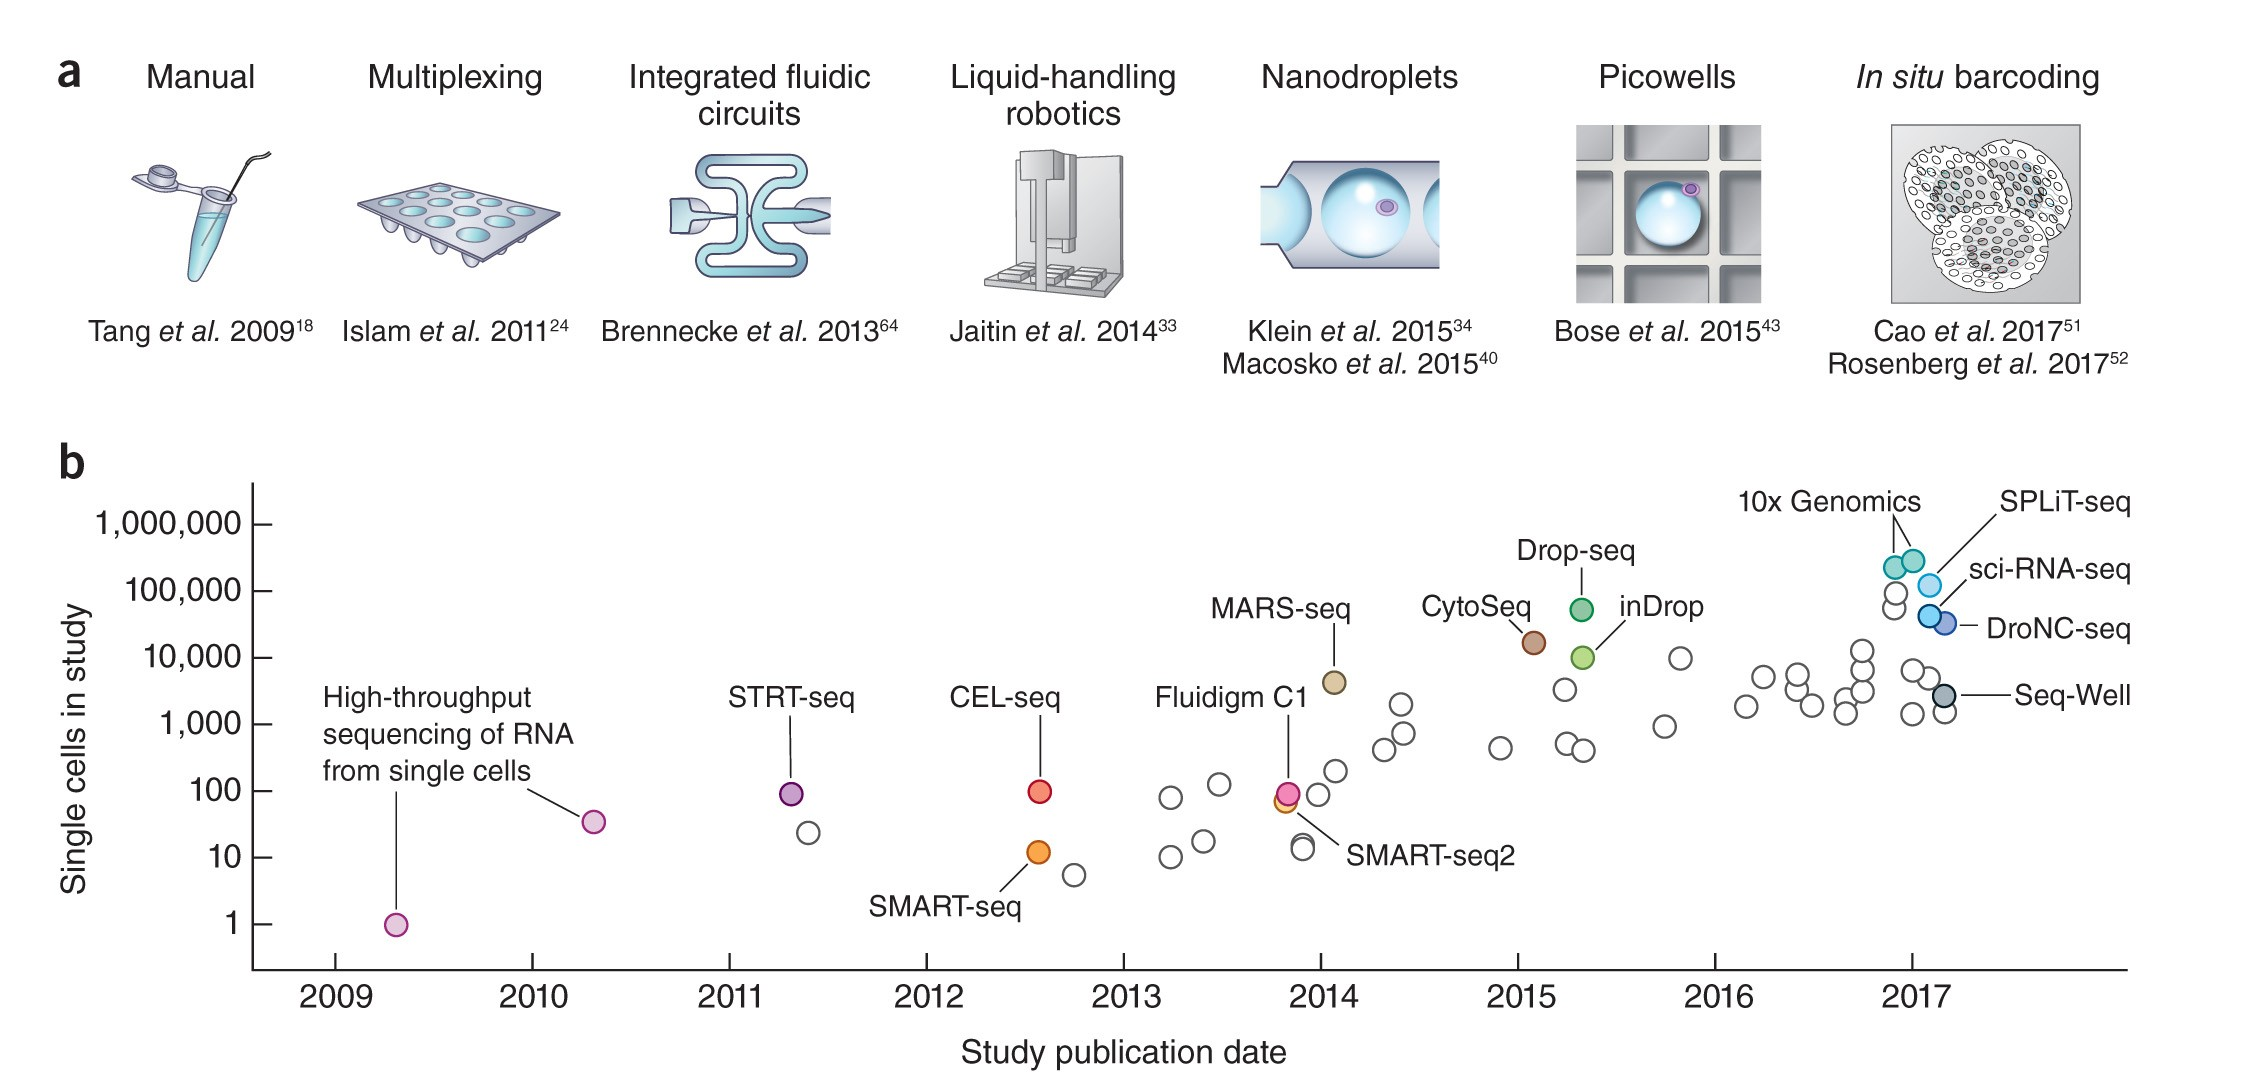
\includegraphics[width=15cm]{Chapter1/Fig/scrnaseq_technologies_svensson2018.jpg}
% \caption[\textbf{scRNA-seq technologies}]{\textbf{Scale of scRNA-seq experiments}.\\
% Technologies that have allowed....

% % make own version adding SmartSeq3 etc 

% adapted from \cite{svensson2018exponential}}
% \label{fig:scrnaseq_technologies}
% \end{figure}

% \subsubsection{Plate-based technologies}

% SmartSeq2

% \subsubsection{Droplet-based technologies}

% DropSeq, 10X Genomics

% \subsubsection{other technologies}

% multi omics aproaches (\cite{stuart2019integrative})

% spatial transcriptomics

% perturb seq

% %\subsection{Analysis of scRNA-seq data}

% \subsection{Computational modelling of scRNA-seq}

% Analysis of scRNA-seq data requires a new set of considerations, largely concerning technical signals, that were not relevant for bulk RNA-sequencing work. 
% Moreover, the resolution of this single-cell data also allows a number of more powerful analysis techniques to be applied.
% This section describes, in brief, how a typical single-cell RNA-sequencing dataset may be analysed.

% \cite{stegle2015computational}

% \subsubsection{Low-level analysis}

% reads QC 

% alignment

% mapping QC

% \subsubsection{Normalisation and batch correction}

% Count matrix
% 10 Genomics: UMI counts
% Smasrtseq2: expected counts or TPM (similar to bulk)

% cell QC (e.g. remove cells with less than xx total counts, yy total genes)
% possibly deal with doublets etc - in our case, donor assignment is also here

% normalisation (account for differences due to read coverage etc)

% log transformation (variance stabilising)

% \textbf{feature selection} (isolate most informative genes, e.g. highly variable genes - HVGs)\\

% genes that behave differently from your expected mean-variance relationship

% optional: centering+scaling - standardising

% batch correction (stronger than normalisation) 
% mutual nearest neighbours (MNN, \cite{haghverdi2018batch}) - and then fastMNN
% canonical correlation analysis (CCA, implemented in Seurat \cite{butler2018integrating}), Stuart et al 2019
% LIGER iNMF (negative matrix factorisation),
% Harmony (\cite{nowotschin2019emergent}) - iterative soft k means (fastest)
% Welch et al 2019, Korsunsky et al 2019


% \subsubsection{Computational analysis}

% \textbf{dimensionality reduction}

% \gls{pca} was first introduced by Pearson over a hundreds years ago (\cite{}, see section 1), yet remains one of the most widely used tools \\

% \textbf{clustering}

% unsupervised\\

% \textbf{pseudotime}

% PCA, diffusion maps\\

% \textbf{DE}

% DESeq, edgeR



% \subsubsection{Visualisation techniques}

% Even after application of a dimension-reduction procedure, a typical dataset will retain more than three biologically important dimensions in its new subspace, which makes visual representation of the data challenging. 

% Transforming high-dimensional data into a human-readable format is therefore an important challenge for single-cell data interpretation.

% scRNA-seq data visualisation techniques used in this thesis: 



% \begin{itemize}
%     \item \gls{pca}
%     \item t-distributed stochastic neighbour embedding (tSNE) \cite{maaten2008visualizing}
%     \item uniform manifold approximation and projection (UMAP) \cite{mcinnes2018umap}
% \end{itemize}


% Workflow packages:

% \begin{itemize}
%     \item scanpy
%     \item scater / scran / Single cell experiment (SCE)
%     \item seurat
%     \item SINCERA
% \end{itemize}




% \subsection{General applications of scRNA-seq in biology}

% Studies of single-cell transcriptomes allow us to directly investigate properties of individual cells, i.e. mRNA abundance. 
% Thus gene regulation is analyzed at the single cell level and, unlike traditional bulk RNA- sequencing, cell-to-cell heterogeneity can be considered.

% By measuring gene expression in development, differentiation, or other responses, we can start to understand cellular phenotypes as well as the regulatory processes that determine these phenotypes. 
% In many experiments cells are sampled at many time points and gene expression is assessed.

 
% \subsubsection{Atlases}

% Human Cell Atlas (HCA)

% The human cell atlas aims to provide a comprehensive reference map of all human cells
% \cite{rozenblatt2017human}
% \subsubsection{Cancer}
% \subsubsection{Immunology}
% \subsubsection{Development}

% developmental trajectories 
% A particular advantage of single-cell methods is the ability to capture cells at various developmental
% stages in a single experiment.

% \subsubsection{lineage tracing}

% \newpage

\subsection{The `resolution revolution'}
\label{sec:scrnaseq}

The first single-cell RNA sequencing (scRNA-seq) experiment was published in 2009, and it involved profiling of only eight cells \cite{tang2009mrna}. 
Seven years later, 10X Genomics released a dataset of 
% more than 
1.3 million cells \cite{102016our}.
All in all, in the last decade, over 1,000 scRNA-seq datasets have been published 
\cite{svensson2018exponential, svensson2019curated, svensson2020single},
using a number of different technologies 
\cite{islam2011characterization, hashimshony2012cel, ramskold2012full, picelli2013smart, sasagawa2013quartz, jaitin2014massively, macosko2015highly,klein2015droplet, gierahn2017seq, zheng2017massively, hagemann2020single}
(\textbf{Fig. \ref{fig:scrnaseq_technologies}}). \\

\begin{figure}[h]
\centering
% 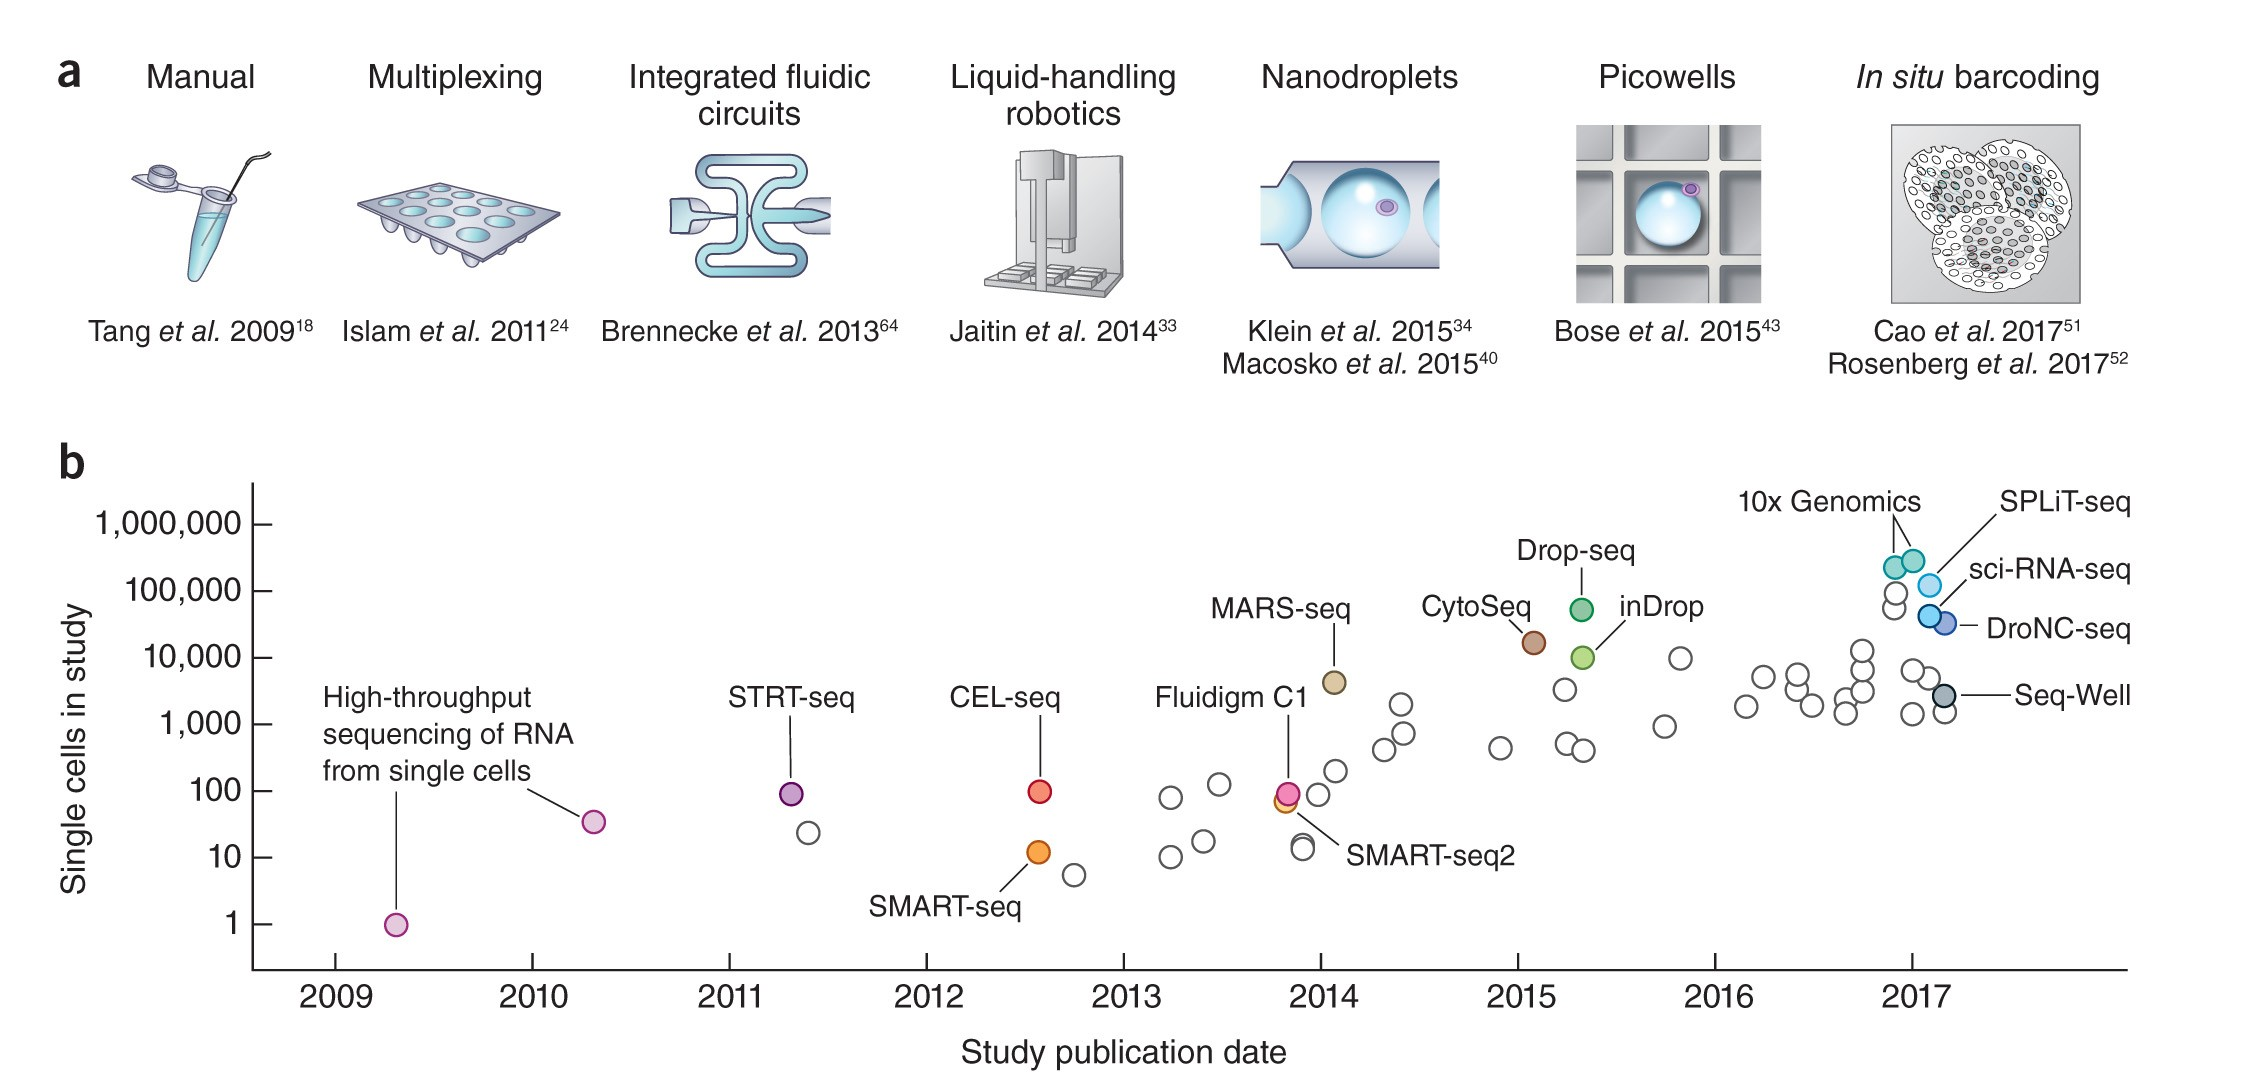
\includegraphics[width=15.5cm]{Chapter1/Fig/scrnaseq_technologies_svensson2018.jpg}
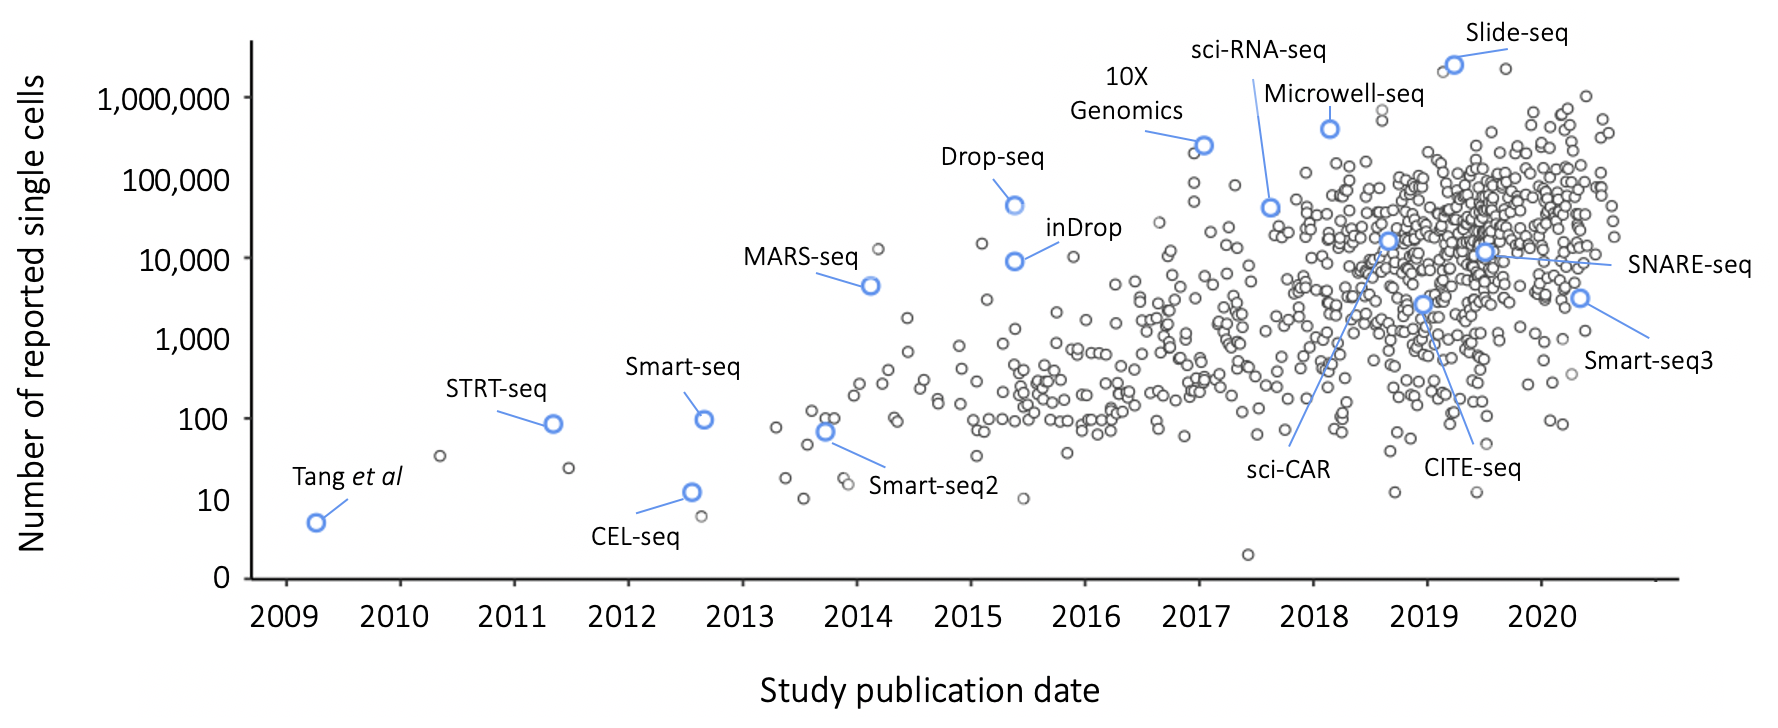
\includegraphics[width=16cm]{Chapter3/Fig/scrnaseq_ncells.png}
\caption[scRNA-seq technologies]{\textbf{Scale of scRNA-seq experiments}.\\
Number of single cells reported in all scRNA-seq publications to date (as collected in \cite{svensson2020single}, y axis), ordered by publication date (x axis).
Key scRNA-seq methods are indicated.
Similar to \cite{svensson2018exponential}.}
\label{fig:scrnaseq_technologies}
\end{figure}

% These methods can be categorised in different ways, but two of the most important aspects are quantification (full-length vs tag-based) and capture (microwell- or plate-, microfluidic-, droplet-based).
% In particular, SmartSeq2 vs 10x used here.
% plate-based: more genes
% droplet-based: more cells\\ 
Single cell RNA-seq protocols differ extensively in terms of scalability, costs and sensitivity 
% % [221, 128] 
\cite{ziegenhain2017comparative, svensson2018exponential}.
However, they can be broadly categorised into methods that are 
% % There are two broad sets of methods for applying single-cell RNA-seq—
`plate-based' or `droplet-based', based on the capture technology used
(\textbf{Fig. \ref{fig:scrnaseq_plate_vs_droplet}}).\\

% From Jonny's thesis
% Initially, most studies used plate-based assays (e.g. SmartSeq), where library preparation is performed manually on cells sorted into and lysed in individual wells of a microwell plate.
% (Figure 1.1) [17, 18].
% Robotic and microfluidic systems (e.g., Fluidigm C1) have been developed to automate some of these processes.
Initially, most studies used plate-based assays, where cells are isolated using micropipettes or flow cytometry into individual wells of a plate, where the library preparation is performed (\textbf{Fig. \ref{fig:scrnaseq_plate_vs_droplet}}).
This class of methods include single-cell tagged reverse transcription sequencing (STRT-seq \cite{islam2011characterization}), Cell Expression by Linear amplification and Sequencing (CEL-seq \cite{hashimshony2012cel}), massively parallel single cell RNA-seq (MARS-seq \cite{jaitin2014massively}) and Smart-seq \cite{ramskold2012full, picelli2013smart, hagemann2020single}. 
\\

% merge below (Jonny + Ricard)
On the other hand, droplet-based methods employ microfluidics to capture individual cells in nanolitre-sized droplets, each loaded with all the necessary reagents for library preparation.
% reagents and unique labels: reverse transcription and transcript labelling take place within these small volumes.
% (Figure 1.1). 
The droplet suspension is later broken down for pooling of cell libraries prior to sequencing (\textbf{Fig. \ref{fig:scrnaseq_plate_vs_droplet}}). 
% Droplet-based methods are based on the use of droplet microfluidics technology [246]. 
% merge below
These methods have been developed by academic groups (InDrop \cite{klein2015droplet} and Drop-seq \cite{macosko2015highly}) and commercially, by 10X Genomics (Chromium \cite{zheng2017massively}). 
These protocols share similar technologies, particularly the use of \glspl{umi} to correct for biases in PCR amplifications \cite{kivioja2012counting}. 
% Differences lie in the barcode design, cDNA amplification step and bead manufacturing [246].
\\

Each approach has its own advantages and disadvantages.
The main advantage of plate-based methods is the higher quality of libraries and, in the case of Smart-seq, the full length transcript information which enables the quantification of splice variants \cite{westoby2018simulation}, allele-specific expression \cite{jiang2017scale} and RNA velocity information \cite{la2018rna}. 
However, this comes at the expense of lower cellular throughput, processing hundreds or thousands of cells compared to the hundreds of thousands that droplet-based methods can achieve.
Indeed, by capturing cells in individual droplets, 
% summarise this
each containing all necessary reagents for library preparation, 
droplet-based protocols allow the profiling of thousands or even millions of cells in a single experiment. 
This, however, comes at the cost of reduced sensitivity.
Additionally, current droplet methods capture gene information exclusively from the 3’ or 5’ end of each transcript, and are more likely to produce `doublets', where two different cells become labelled with the same barcode (\textbf{Fig. \ref{fig:scrnaseq_plate_vs_droplet}}). 
% In contrast, the main drawback lies on the low throughput.
% Yet, multiplexing techniques and the addition of molecular barcodes to cDNA fragments allow the parallel processing of multiple experiments, thereby increasing the scale of each experiment.
% As a trade-off, the increased high throughput of droplet-based approaches 
% [252, 238, 222] (Figure 1.1).
% Each approach has its own advantages and disadvantages.
% Plate-based methods tend to provide higher-quality libraries at the cost of lower cellular throughput, processing hundreds or thousands of cells compared to the hundreds of thousands that droplet methods can achieve.
% summarise below
% More subtle differences also differentiate the two sets of methods. 
% To capture rare cell types with known cell-surface markers, it is generally more efficient to flow-sort and prepare plates of single-cell libraries rather than the brute-force approach of capturing more cells outright using a droplet method. 
% Additionally, current droplet methods capture gene information exclusively from the 3’ or 5’ end of each transcript, while some plate approaches generate reads from across entire transcripts; the latter allows splice-variant and allele-specific transcriptional information to be retrieved. 
% Finally, droplet methods are more likely to produce `multiplet' cell transcriptomes, where multiple different cells become labelled with the same barcode. 
% This is largely due to the lack of user oversight (e.g., it is more difficult to identify attached pairs of cells) and the possible reuse of cell barcodes from the labelling beads. 
% The doublet rate in droplet experiments is proportional to the number of loaded cells [21]; hence a user may reduce the rate of this confounding, albeit by sacrificing cost-efficiency, by loading fewer cells per sample.
\\

\begin{figure}[h]
\centering
% 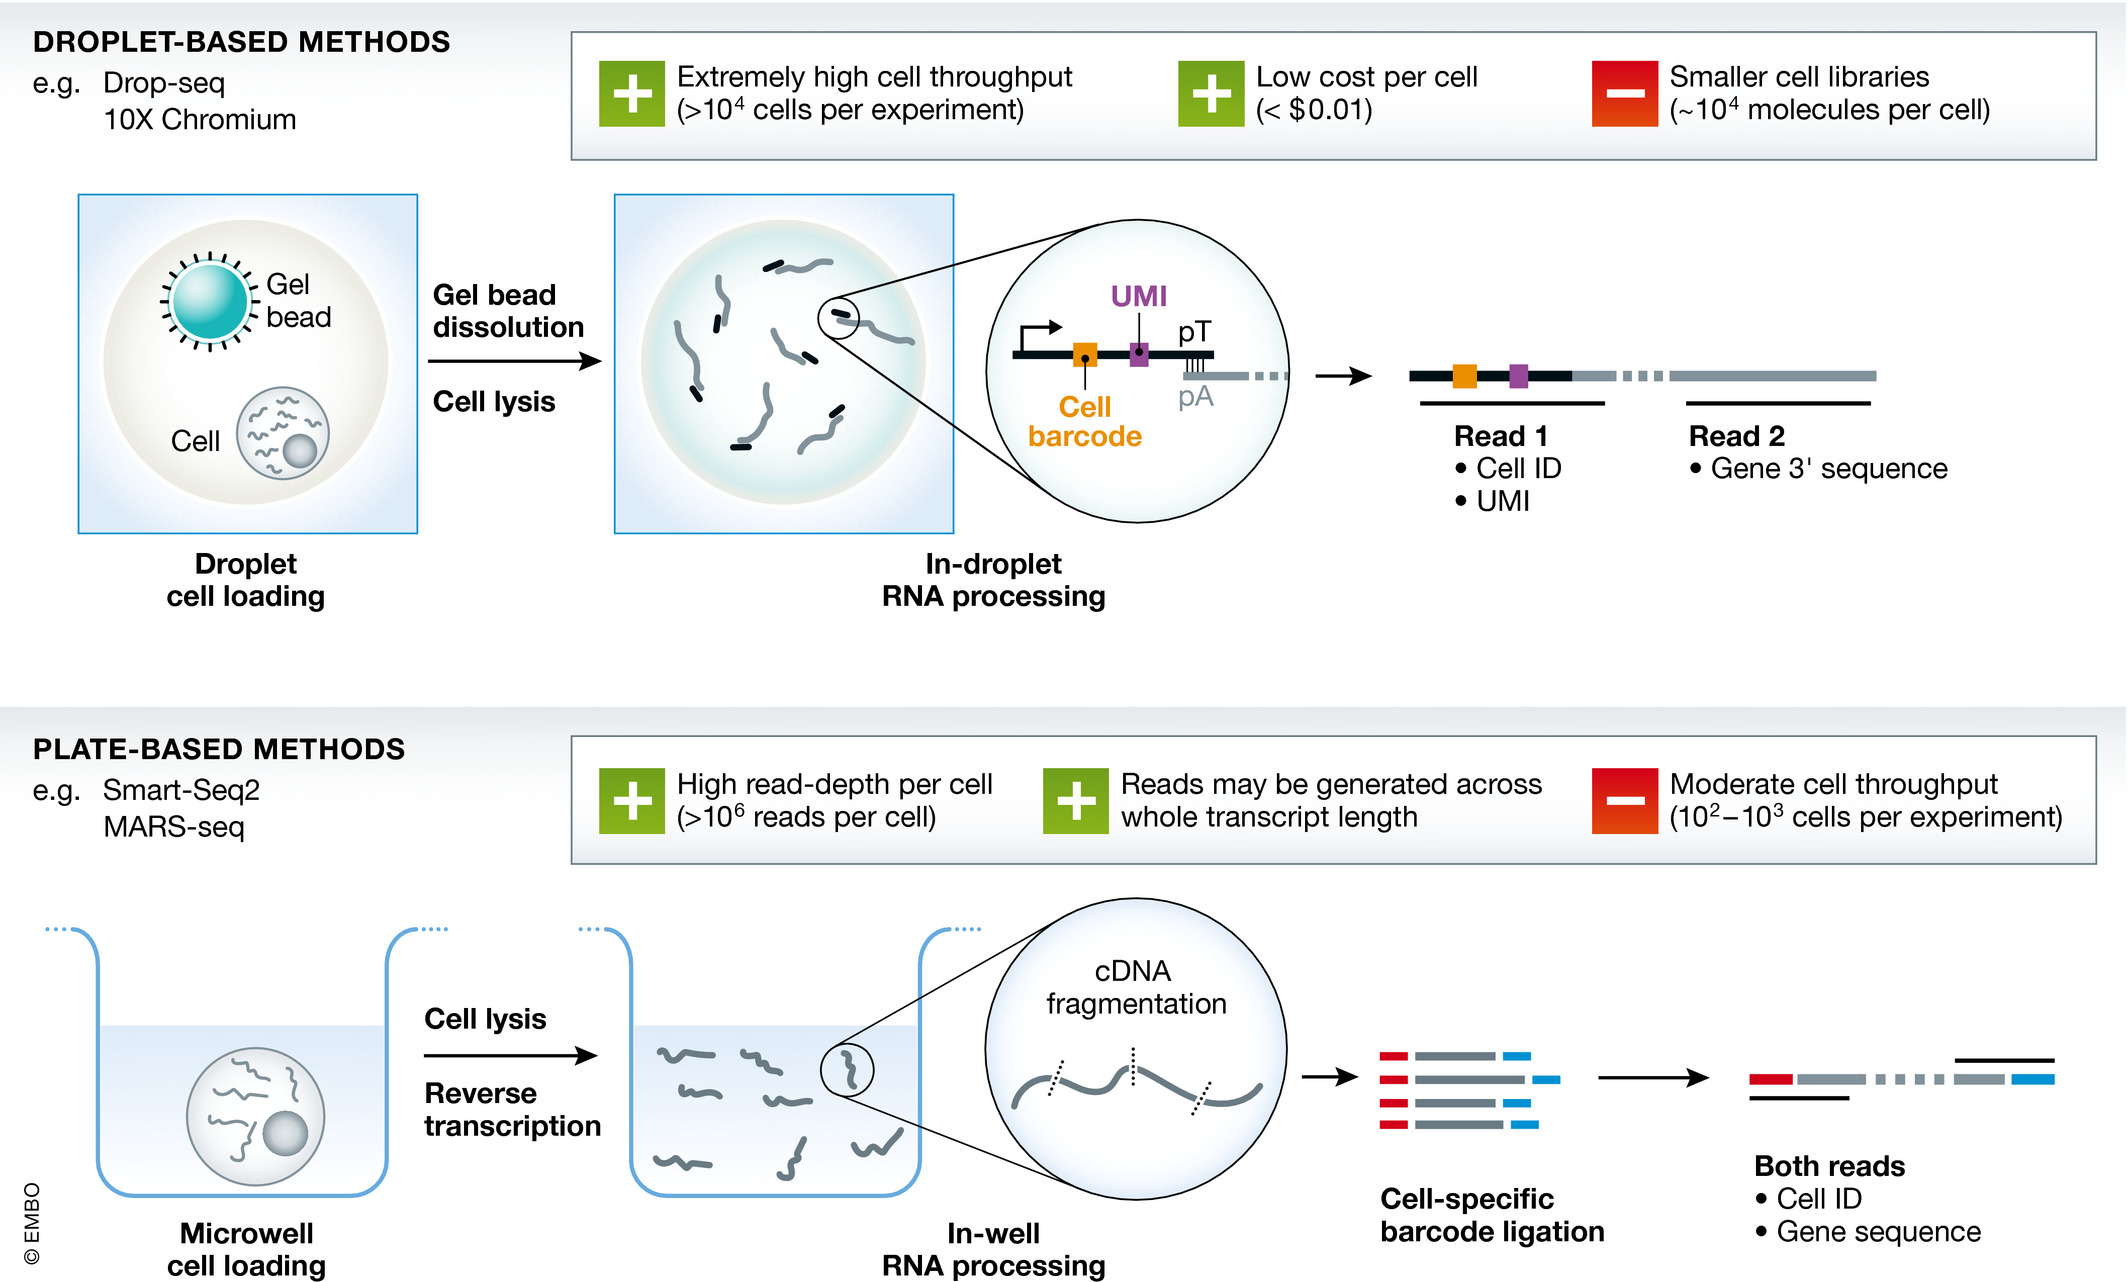
\includegraphics[width=14.5cm]{Chapter3/Fig/plate_vs_droplet_griffiths2018.jpg}
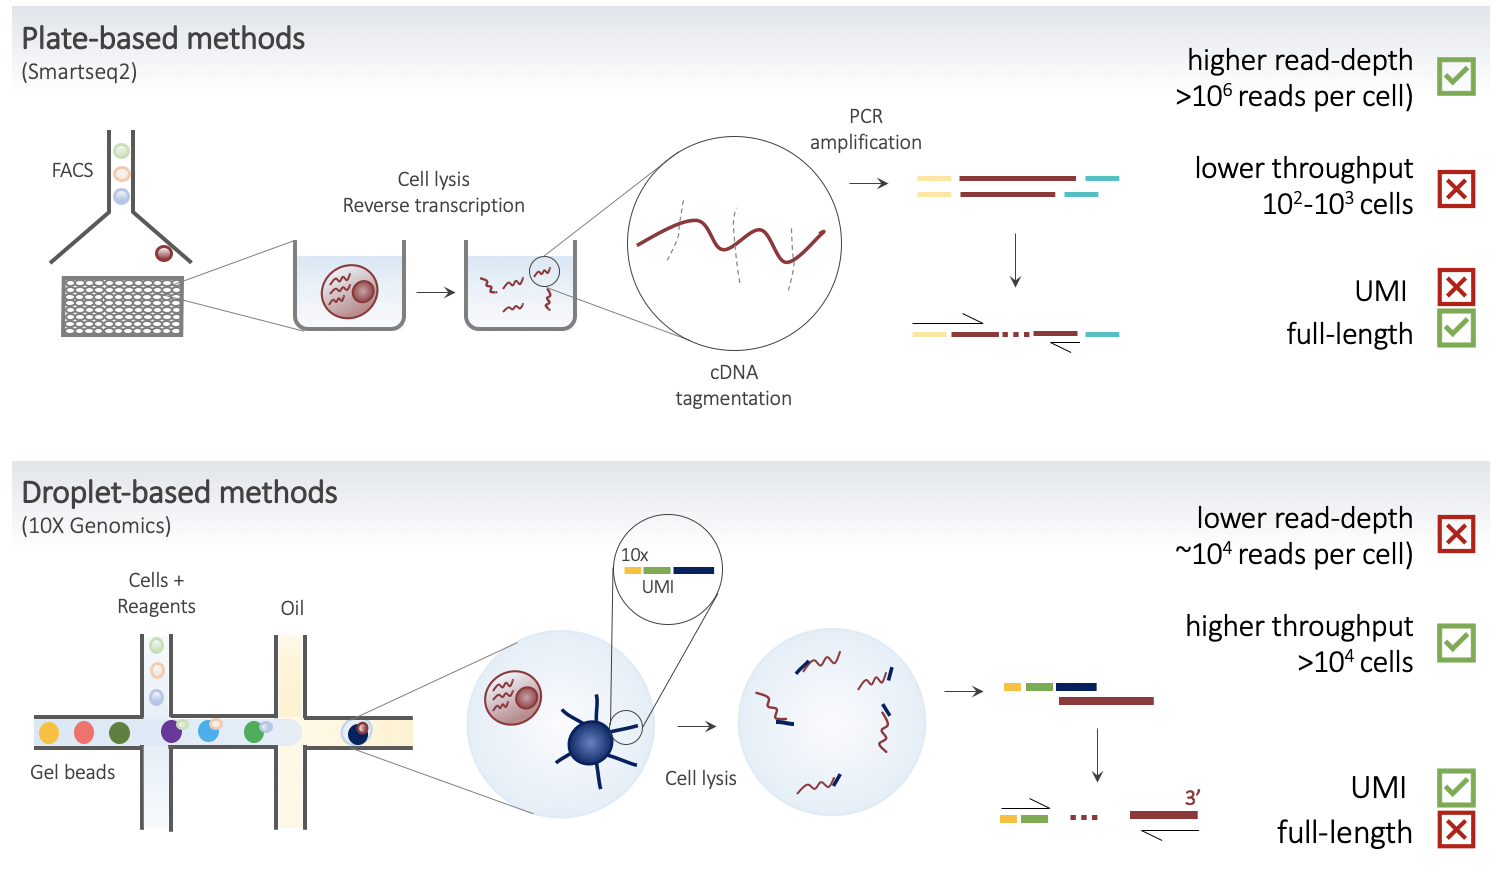
\includegraphics[width=16cm]{Chapter3/Fig/plate_vs_droplet.png}
\caption[scRNA-seq plate vs droplet]{\textbf{Plate-based vs droplet-based methods for scRNA-seq}.\\
An illustration of the key differences between plate-based methods (exemplified by SmartSeq2 \cite{picelli2013smart}) and droplet-based methods (represented by 10X Genomics Chromium \cite{zheng2017massively}).
The key trade-off is between the cell-throughput (much higher for droplet-based methods) and the read-depth per cell (higher for plate-based methods).
Additionally, the full-length transcripts obtained using SmartSeq2 allow quantification of allele-specific expression and splice variants, which are not possible with 3' tag 10X data.
Finally, all droplet-based methods include UMI, which allow the robust quantification of PCR duplicates.

Note that these last two differences (in terms of UMIs and full length) specifically hold true for the two methods shown here (and used in this thesis: SmartSeq2 and 10X Genomics).
Indeed, not all plate-based methods provide full-length transcript information (e.g. MARS-seq \cite{jaitin2014massively} and CEL-seq \cite{hashimshony2012cel} do not).
In contrast, the most recent SmartSeq3 \cite{hagemann2020single} can include UMIs, despite being a plate-based method.
Figure similar to \cite{griffiths2018using}.}
\label{fig:scrnaseq_plate_vs_droplet}
\end{figure}

% \newpage

% Analysis of scRNA-seq data requires a new set of considerations, largely concerning technical signals, that were not relevant for bulk RNA-sequencing work.
% Moreover, the resolution of this single-cell data also allows a number of more powerful analysis techniques to be applied.
% This section describes, in brief, how a typical single-cell RNA-sequencing dataset may be analysed.
In the last 10 years, technological improvement (\textbf{Fig. \ref{fig:scrnaseq_technologies}}) has gone hand-in-hand with computational advances to analyse the resulting data, which require a new set of considerations that were not relevant for bulk RNA-seq data.
% maybe highlight that droplet-based method are more and more popular
% Today, scRNA-seq is an established technique
Indeed, to complement the explosion of scRNA-seq studies published, an entire ecosystem of computational methods for analysing them has emerged.
% \\ 
% (add figure/table?) 
In some cases, those methods have been directly borrowed from bulk RNA-sequencing methods; other times, methods tailored specifically for single cell data were proposed \cite{stegle2015computational, zappia2018exploring, luecken2019current}.
% \\

\clearpage

Single cell-specific bioinformatics workflows such as Cell Ranger \cite{zheng2017massively}, indrops \cite{klein2015droplet}, SEQC  \cite{azizi2018single}, or zUMIs \cite{parekh2018zumis}
have been developed to perform 
% the very first 
raw data processing tasks,
% by
% pipelines such as 
% for example 
% .
% Namely, these 
i.e. read-level QC, assignment of reads to their cell barcodes and mRNA molecules of origin (i.e. `demultiplexing'), alignment to the reference genome, and quantification. 
Additional methods allow the assignment of cells to their donor of origin, in case of  multi-individual pooled designs \cite{kang2018multiplexed, mccarthy2020cardelino}.
% Generating single‐cell data from a biological sample requires multiple steps. Typical workflows incorporate single‐cell dissociation, single‐cell isolation, library construction, and sequencing
% After the alignment of the sequencing reads to a reference genome, 
The data resulting from a scRNA-seq experiment are typically represented as an integer matrix of gene expression levels, with entries representing the number of sequenced reads (or molecules, if UMIs were used) assigned to a particular gene in a specific cell \cite{griffiths2018using}.
Starting from these count matrices, a common scRNA-seq analysis workflow may be divided into pre-processing steps and downstream analysis \cite{luecken2019current} - and scRNA-seq-specific tools have been implemented for several of the steps along the pipeline.\\

In particular, methods have been proposed to perform  cell calling, i.e. to detect, and exclude, empty droplets \cite{lun2019emptydrops}, doublets \cite{wolock2019scrublet, mcginnis2019doubletfinder, depasquale2018doubletdecon}, and ambient RNA \cite{young2020soupx}.
% Next, standard cell QC steps involve ..
% The distributions of these QC covariates are examined for outlier peaks that are filtered out by thresholding
% cell QC (number of reads, genes, MT, most expressed)
Moreover, methods for normalisation have been described in \cite{lun2016pooling, vallejos2017normalizing, weinreb2018spring}.
% CPM
% Thus, when gene expression is compared between cells based on count data, any difference may have arisen solely due to sampling effects. Normalisation addresses this issue by e.g. scaling count data to obtain correct relative gene expression abundances between cells.
% normalisation, size factors (UMI?)
% Add normalisation.
After normalisation, data matrices are typically log(x+1)‐transformed. 
Additionally, several novel methods allow to correct for confounding factors including batch effects \cite{haghverdi2018batch, butler2018integrating, nowotschin2019emergent, stuart2019comprehensive, welch2019single, polanski2020bbknn} and
cell cycle effects \cite{scialdone2015computational, mcdavid2016reply}.
To ease the computational burden on downstream analysis tools, reduce the noise in the data, and to visualise the data, one can use several approaches to reduce the dimensionality of the dataset.
First, feature selection, for example by detecting highly variable genes (HVGs) \cite{brennecke2013accounting, yip2019evaluation}.
Next, dimensionality reduction is performed either using linear methods, such as \gls{pca}, or non-linear methods, with the latter being preferred for visualisation purposes.
In particular, t-distributed stochastic neighbour embedding (tSNE)  \cite{maaten2008visualizing} and uniform manifold approximation and projection (UMAP) \cite{mcinnes2018umap} are extremely popular (for a review of other methods, see \cite{moon2018manifold}). 
Downstream analysis methods can be classified into cell-level and gene-level.
The former include clustering \cite{kiselev2017sc3, traag2019louvain}, often followed by cell type annotation \cite{kiselev2018scmap}, as well as pseudotime inference \cite{haghverdi2016diffusion, trapnell2014dynamics, bendall2014single, wolf2019paga}.
Finally, single cell-specific methods have been developed for gene-level analyses, including differential expression analysis \cite{finak16others}, and gene regulatory networks identification \cite{matsumoto2017scode, chan2017gene, aibar2017scenic}.\\


% such as read alignment, cell calling and visualisation \cite{maaten2008visualizing, mcinnes2018umap} as well as to perform higher level tasks such as batch correction \cite{haghverdi2018batch, butler2018integrating, nowotschin2019emergent, stuart2019comprehensive, welch2019single, polanski2020bbknn}, clustering \cite{kiselev2017sc3, traag2019louvain} and pseudotime inference \cite{haghverdi2016diffusion}.\\

A typical workflow for single cell RNA-seq data implemented in R can be found on Bioconductor\footnote{at \url{https://bioconductor.org/packages/devel/bioc/vignettes/scran/inst/doc/scran.html} and

\url{https://osca.bioconductor.org}} using scRNA-seq specific R packages scran \cite{lun2016step, risso2016scrnaseq}, scater \cite{mccarthy2017scater}, and SingleCellExperiment 
\cite{lun2019singlecellexperiment}.
Other pipelines for scRNAseq data analysis include 
Seurat \cite{butler2018integrating},
Scanpy \cite{wolf2018scanpy}, 
and SINCERA \cite{guo2015sincera}. 
% \\


% \begin{figure}[htbp]
% \centering
% 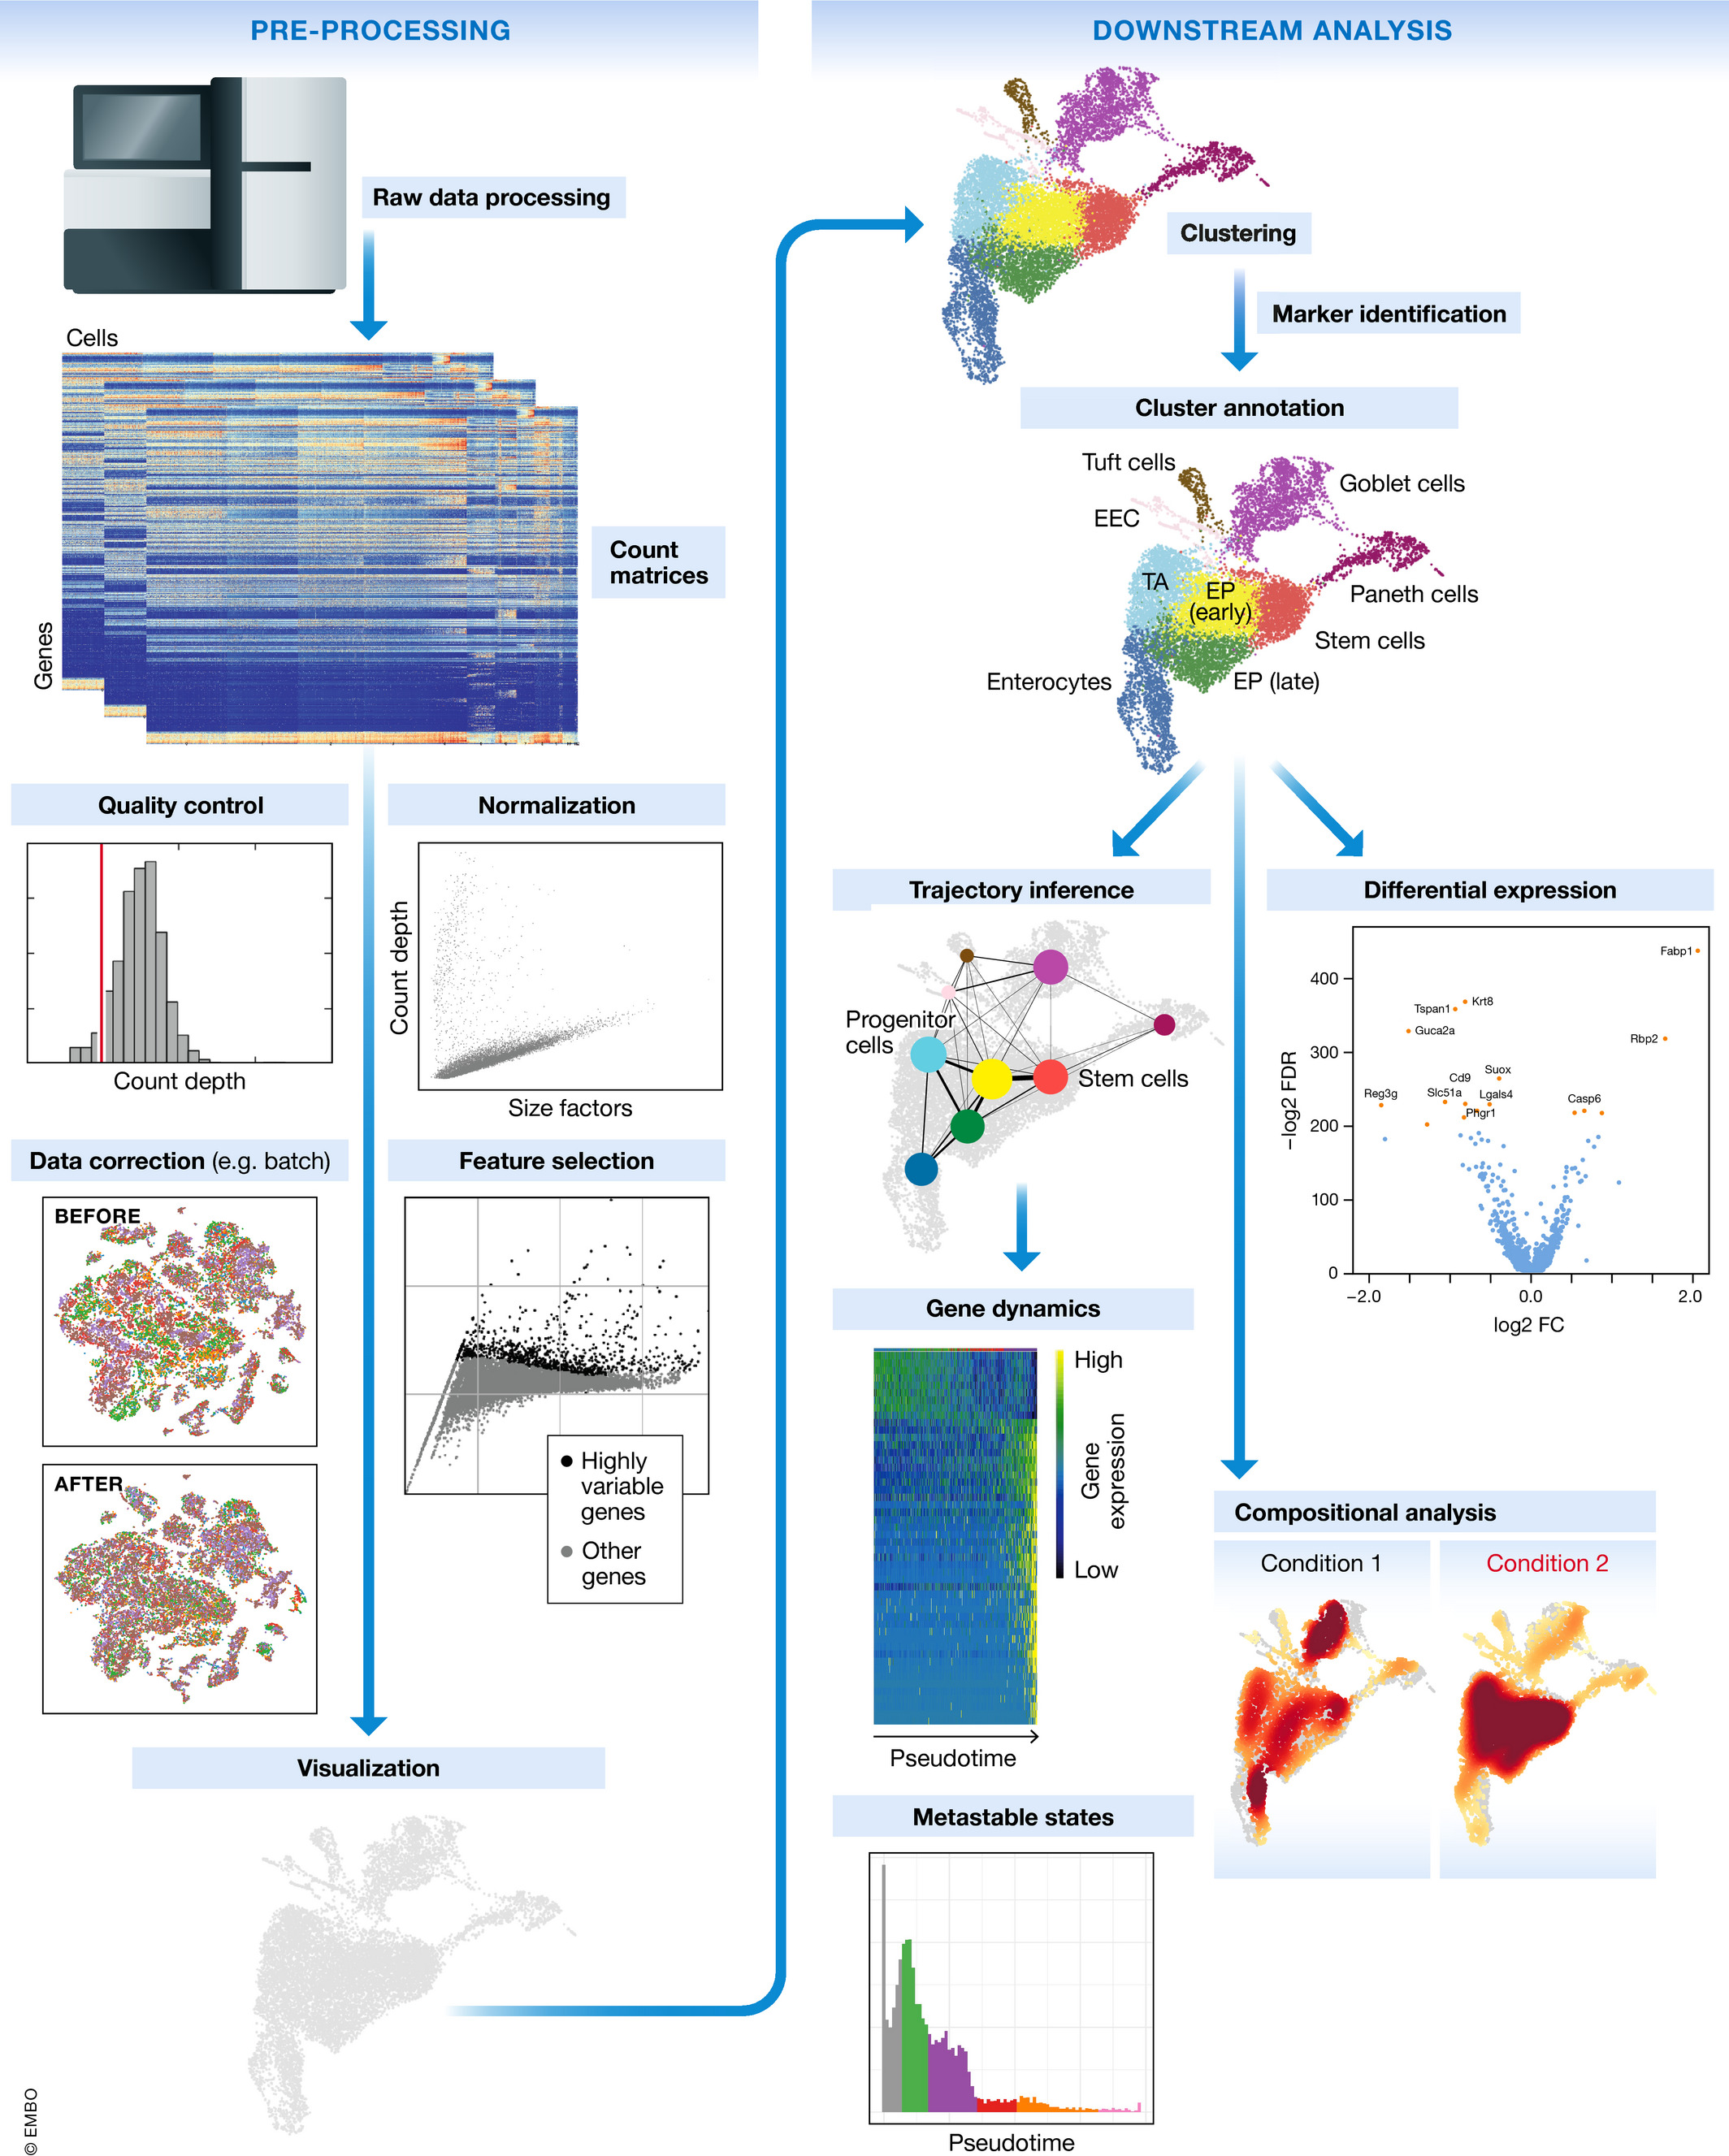
\includegraphics[width=14.5cm]{Chapter3/Fig/scrnaseq_analysis_luecken2019.jpg}
% \caption[scRNA-seq analysis pipeline]{\textbf{scRNA-seq analysis pipeline}.\\
% % (make own version)
% Adapted from \cite{luecken2019current}}
% \label{fig:scrnaseq_analysis_pipeline}
% \end{figure}

% Here I will only mention a few key steps.



% \subsubsection{Low-level analysis}
% reads QC 
% alignment
% mapping QC

% cell QC (e.g. remove cells with less than xx total counts, yy total genes)
% possibly deal with doublets etc - in our case, donor assignment is also here
% normalisation (account for differences due to read coverage etc)
% log transformation (variance stabilising)

% feature selection (isolate most informative genes, e.g. highly variable genes - HVGs)
% genes that behave differently from your expected mean-variance relationship



% Several platforms implement the entire processing workflow, or at least large portions of it.
% These include R packages seurat \cite{stuart2019comprehensive} and SINCERA (SINgle CEll RNA-seq profiling Analysis, \cite{guo2015sincera}) and python package scanpy \cite{wolf2018scanpy}. 



% \subsection{Computational modelling of scRNA-seq}

% Analysis of scRNA-seq data requires a new set of considerations, largely concerning technical signals, that were not relevant for bulk RNA-sequencing work. 
% Moreover, the resolution of this single-cell data also allows a number of more powerful analysis techniques to be applied.
% This section describes, in brief, how a typical single-cell RNA-sequencing dataset may be analysed.



% \subsubsection{Normalisation and batch correction}

% Count matrix
% 10 Genomics: UMI counts
% Smartseq2: expected counts or TPM (similar to bulk)



% \textbf{feature selection} (isolate most informative genes, e.g. highly variable genes - HVGs)\\

% genes that behave differently from your expected mean-variance relationship

% optional: centering+scaling - standardising

% batch correction (stronger than normalisation) 
% mutual nearest neighbours (MNN, \cite{haghverdi2018batch}) - and then fastMNN
% canonical correlation analysis (CCA, implemented in Seurat \cite{butler2018integrating}), Stuart et al 2019
% LIGER iNMF (negative matrix factorisation),
% Harmony (\cite{nowotschin2019emergent}) - iterative soft k means (fastest)
% Welch et al 2019, Korsunsky et al 2019


% \subsubsection{Computational analysis}

% \textbf{dimensionality reduction}

% \gls{pca} was first introduced by Pearson over a hundreds years ago (\cite{}, see section 1), yet remains one of the most widely used tools \\

% \textbf{clustering}

% unsupervised\\

% \textbf{pseudotime}

% PCA, diffusion maps\\

% \textbf{DE}

% DESeq, edgeR



% \subsubsection{Visualisation techniques}

% Even after application of a dimension-reduction procedure, a typical dataset will retain more than three biologically important dimensions in its new subspace, which makes visual representation of the data challenging. 

% Transforming high-dimensional data into a human-readable format is therefore an important challenge for single-cell data interpretation.

% scRNA-seq data visualisation techniques used in this thesis: 



% \begin{itemize}
%     \item \gls{pca}
%     \item t-distributed stochastic neighbour embedding (tSNE) \cite{maaten2008visualizing}
%     \item uniform manifold approximation and projection (UMAP) \cite{mcinnes2018umap}
% \end{itemize}

\newpage

\subsection{Single cell eQTL mapping}
\label{sec:sc_eqtl}

With the ability to identify cell types and states in an unbiased manner \cite{kolodziejczyk2015technology, trapnell2015defining}, the use of 
% population-scale 
scRNA-seq data, combined with genotype information, is uniquely positioned to provide an extra layer 
of information on the regulatory role of common genetic variants
% (including disease-associated variants) 
on
% to our understanding of the genetic regulation of 
gene expression, across a plethora of cell types and states.
As a consequence, single cell \gls{eqtl} mapping 
% has emerged as a field, 
is increasingly feasible,
% as the cost of sequencing reduces,
and promises to improve our understanding of genetic regulation both in health and disease across tissues \cite{wills2013single, van2018single, sarkar2019discovery, jerber2020population, van2020single1, cuomo2020single}.
\\

When performing \gls{eqtl} mapping using scRNA-seq profiles, a first important step is to verify the feasibility of traditional `mean level' \gls{eqtl} mapping, i.e. to reproduce \glspl{eqtl} previously identified using bulk RNA-seq.
Only then can we explore new avenues and alternative types of \gls{eqtl} analyses, which are especially enabled by the single cell resolution (\textbf{Fig. \ref{fig:sc_eqtl}}).\\

\begin{figure}[h]
\centering
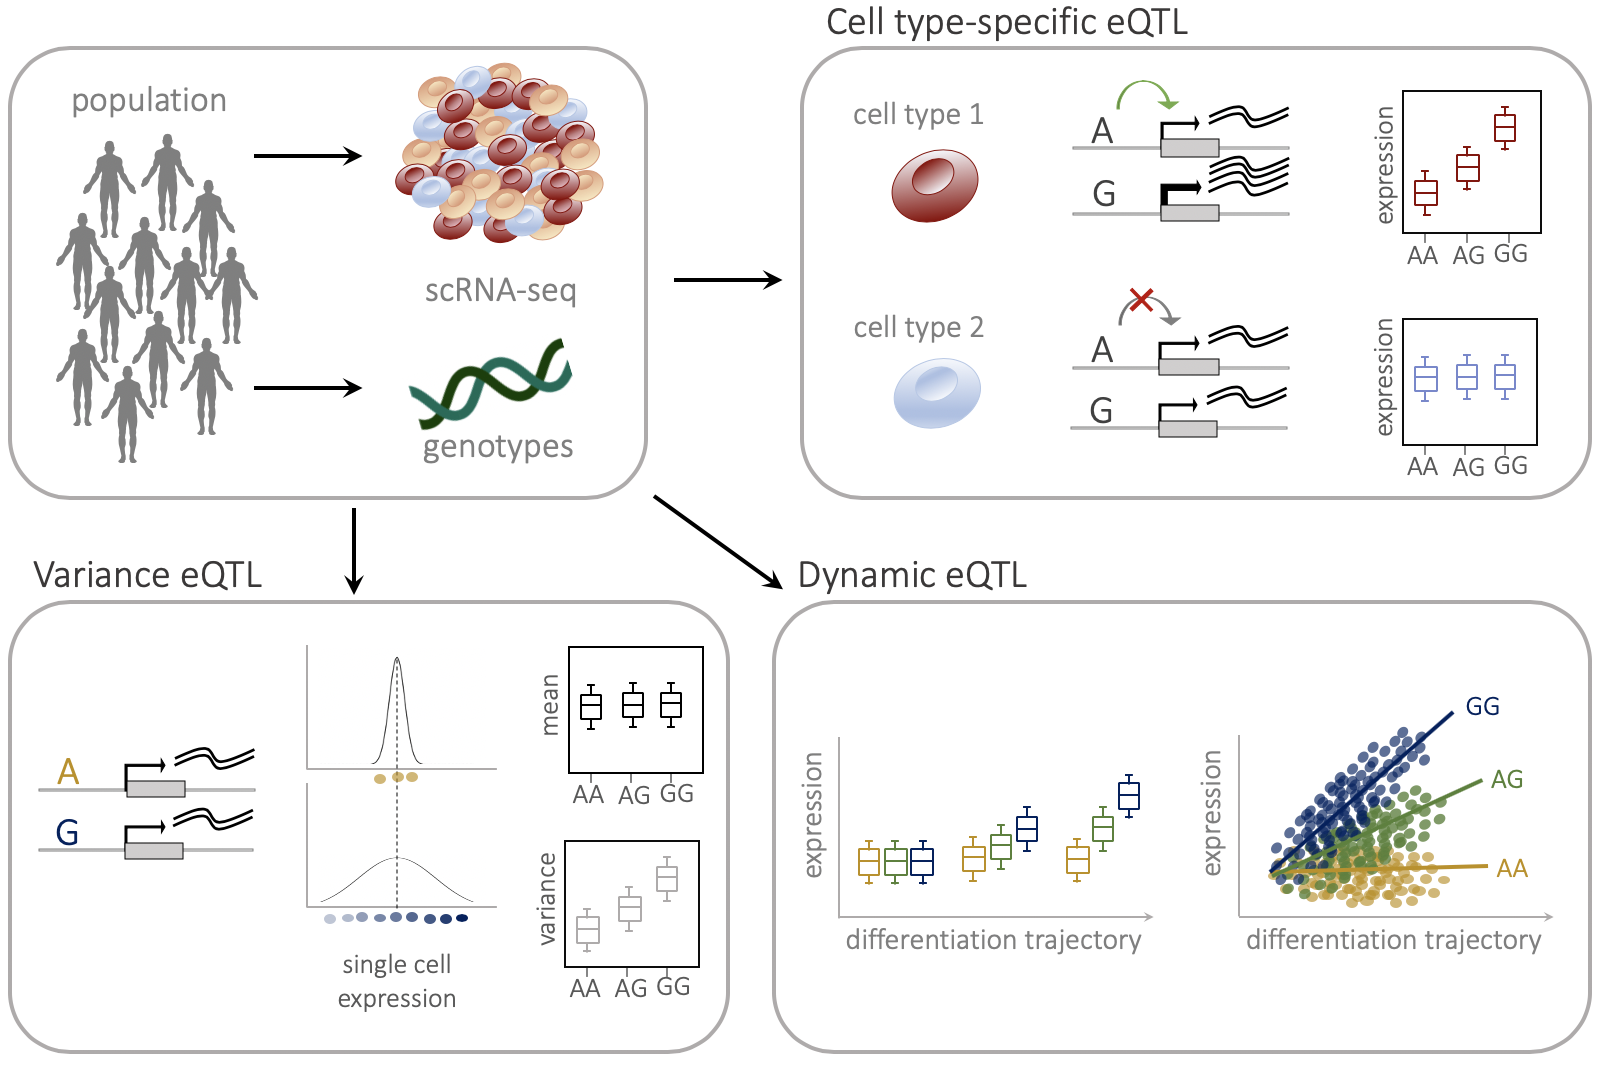
\includegraphics[width=14cm]{Chapter3/Fig/sc_eqtl.png}
\caption[Single cell eQTL]{\textbf{Overview of single cell eQTL mapping methods}.\\
Matched genotypes and scRNA-seq data from several individuals allow the detection of cell type-specific \gls{eqtl}, variance \gls{eqtl} (genetic effects on cell-to-cell transcriptional variability), and dynamic \gls{eqtl} (dynamic genetic effects along cellular differentiation or other cellular states).}
\label{fig:sc_eqtl}
\end{figure}

In this chapter, we address the first point (i.e. mapping mean-level sc-\gls{eqtl}).
To do so, we leverage bulk and single cell gene expression of matched human 
% \gls{ipsc}
iPSC
lines from around 100 donors to identify general guidelines for \gls{eqtl} mapping using scRNA-seq data.
% We compare several manners of normalising and aggregating expression across cells per donor as well as different models to test for \gls{eqtl} and compare to equivalent results obtained when using bulk RNA seq data.
% Whilst for most individuals we have plate-based sc-RNAseq data (SmartSeq2, \cite{picelli2013smart}), we also have data using the 10X Genomics platform \cite{zheng2017massively} for a subset of around 30 samples, which allows us - to an extent - to also compare results across single cell technologies.

\newpage

\section{What is different in single cell data?}
% \section{What can we learn from single cell data?}

When we perform \gls{eqtl} mapping, we are interested in finding differences in expression level between individuals, when stratified by their genotypes at a genomic locus of interest (\textbf{page 
\pageref{fig:eqtl}}). 
Under the assumption that we are looking at an otherwise homogeneous population of cells (e.g. all cells are from the same cell type), it is reasonable to consider the total (or the average) expression for each individual and gene, across all cells.
When we use bulk RNA sequencing expression profiles, that is essentially what happens: all cells from an individual are pooled, the mRNA is extracted, reverse-transcribed to cDNA, and then sequenced. 
The resulting reads are then mapped onto a reference genome, and the expression level of each gene is quantified as the number of reads (raw counts) obtained from one donor that uniquely map to that gene, after normalisation, e.g. transcripts per million (TPM)\footnote{i.e. for every 1,000,000 RNA molecules in the RNA-seq sample, x came from this gene/transcript.}. 
A bulk RNA-seq experiment, therefore, results in one individual measure of `abundance' of each gene for each donor. 
Such a measure results in 
% measure is the results of 
aggregating over 
hundreds of thousands of cells
% XX-YY cells (ZZ on average, \cite{})
and, at least for expressed genes (e.g. average TPM > 1), the vector of gene expression across individuals follows a distribution that can be approximated as Gaussian \cite{piras2015reduction}.
% \\
% The intuition here is that 
% Pool of RNA transcripts from many genes (low probability for a given gene), get a sample to sequence. 
% Poisson: sampling from large n, small p (samples are technical replicates)
% (biological replicates - NB > Poisson, larger variance )
% As discussed,
% % in section 1.3 of the Introduction, 
% robust experimental methods are now available to assay expression profiles of individual cells, using scRNA-seq.
% , allowing to assay the genome-wide transcriptome of hundreds to thousands of individual cells. 
On the other hand,
whilst scRNA-seq data provides increased resolution and promises great insights into cellular function, the data are also much sparser, and the number of cells that can be assayed for an individual is limited compared to bulk (often as little as 10-100 cells). 
In addition, the number of cells that can be assessed often varies substantially from individual to individual.
As a result, the distribution of total counts from a single cell experiment as opposed to its corresponding bulk experiment has lower mean (fewer cells, fewer reads, \textbf{Fig. \ref{fig:sc_bulk_counts}}) and higher variance (due to the variable number of cells across donors, \textbf{Fig. \ref{fig:sc_bulk_counts}} vs \textbf{Fig. \ref{suppl_fig:counts_sc_ncells}}).
% (on average XX compared to YY for bulk RNA-seq, \cite{}).
% Moreover, in addition to observing a smaller number of cells (and therefore total reads) for an individual as compared to bulk, the read distribution typically does not follow a normal distribution, mostly due to very different amounts of reads coming from different donors. \\

\begin{figure}[h]
\centering
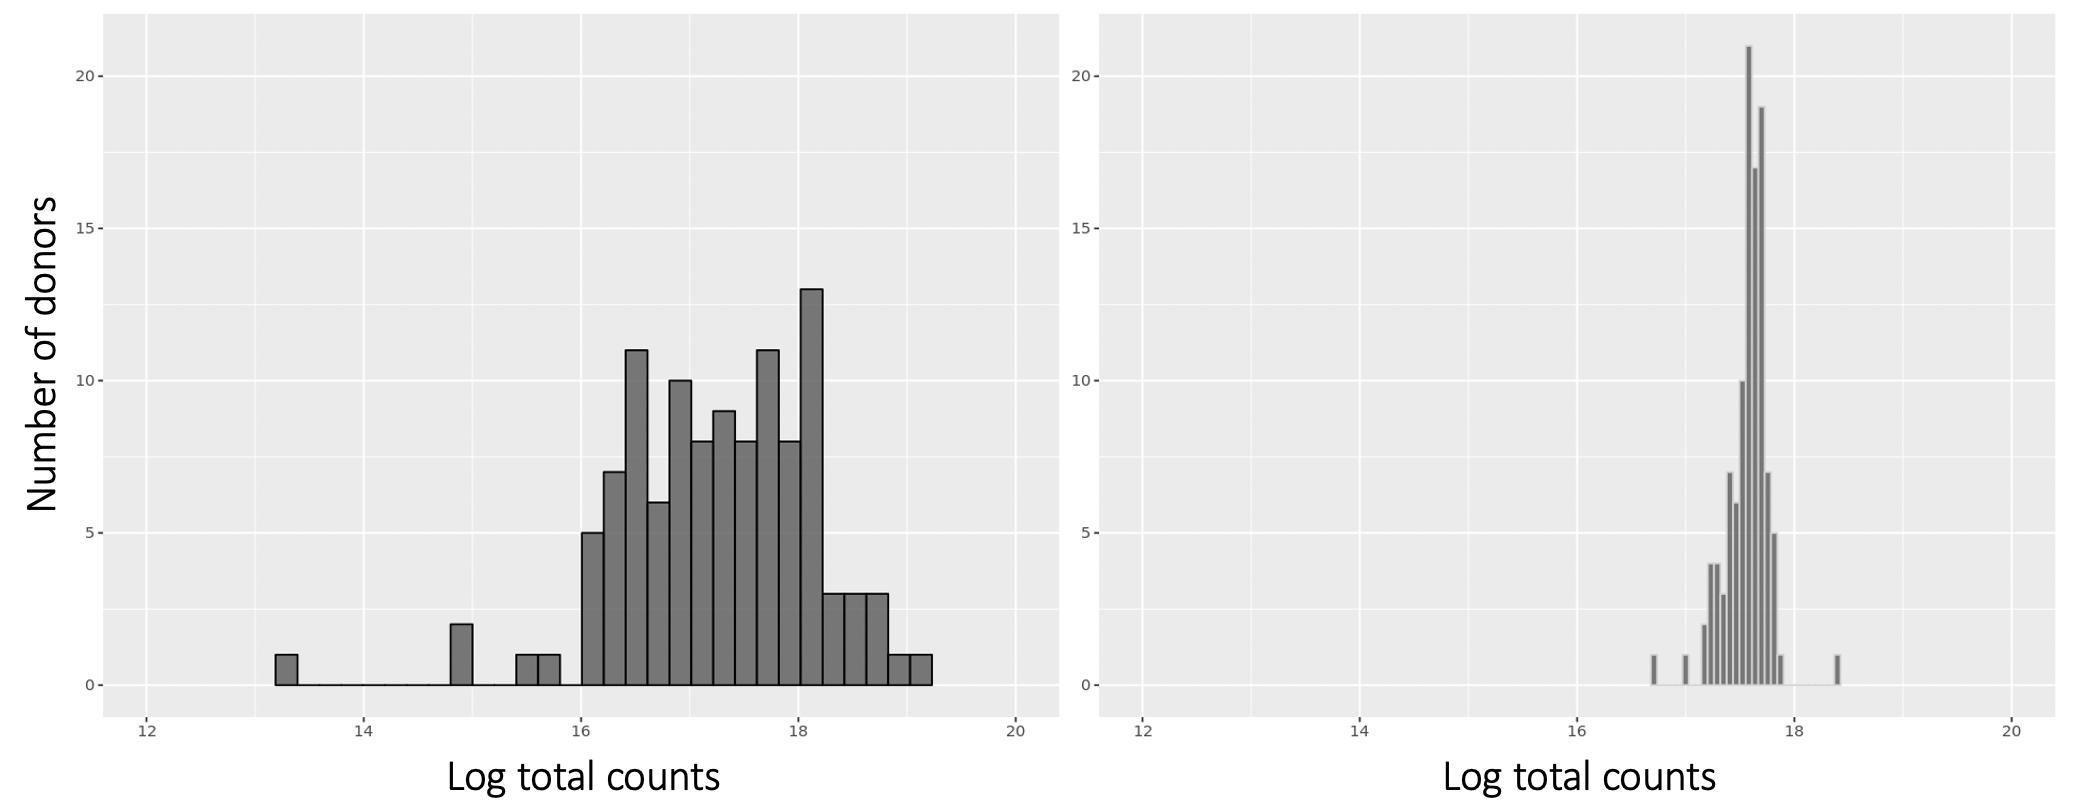
\includegraphics[width=13cm]{Chapter3/Fig/count_distribution_sc_vs_bulk.png}
\caption[Distribution of reads]{\textbf{Distribution of reads}.\\
Distribution of total reads (across all genes) per individual for matched 
% \gls{ipsc}
iPSC
data (108 individuals) using single cell (left, from \cite{cuomo2020single}) and bulk (right, from \cite{mirauta2018population}) RNA-seq data.}
\label{fig:sc_bulk_counts}
\end{figure}
% This is in part due to the `double sampling' that is inherent of the technology: there is a chance of not sampling any reads from one gene in one cell, and there is a chance of not sequencing any reads from that cell at all.

% Add differences in number of total reads, read distribution, describe “double sampling” process.

\newpage

% \section{Data}
\section{Single cell and bulk RNA-seq profiling of iPSCs}

The data I use in this chapter to benchmark methods for single cell \gls{eqtl} mapping 
% were generated by colleagues at the Sanger Institute
% % \footnote{The Ludovic Vallier lab, at the Wellcome Trust Sanger Institute, Cambridge, UK.
% % Full acknowledgments and contributions for this project can be found in the next chapter, at page \pageref{contr:chapter4}.}
% , using human \gls{ipsc} lines from the
% HipSci
% % \gls{hipsci} 
% resource (see section 
% % \ref{sec:ips_genetics}).
% 1.2.6). 
% They 
were generated as part of a larger study, where \gls{ipsc} lines from over 100 donors (from HipSci) are differentiated towards definitive endoderm.
A pooled design was adopted, where cells from 4-6 lines were differentiated together, to avoid for individual genetic differences to be confounded with batch variation. 
Cells were later assigned to their donor of origin using Cardelino \cite{mccarthy2020cardelino}. 
Next, cells were collected at four time points (day0, day1, day2, day3) and sequenced using Smartseq2 \cite{picelli2013smart}, a plate-based single cell technology (\textbf{Fig. \ref{fig:scrnaseq_plate_vs_droplet}}).
This study was published earlier this year \cite{cuomo2020single}, and I discuss the key results from it in the next chapter (\textbf{Chapter 
\ref{chapter4}}).
% 4}).
\\

% In this chapter, 
Here,
I focus on the earliest time point (i.e. day0), where cells are still pluripotent, prior to cell differentiation.
We expect iPS cells to be fairly homogeneous, so it is the ideal cell type to use to perform this kind of study.
After QC\footnote{Some QC steps were performed for all time points jointly, therefore I refer the reader to the detailed QC pipeline described in the next chapter, at \textbf{page \pageref{fig:endodiff_qc_workflow}}.}, data was available from 9,661 iPS cells and 11,231 genes, from 112 unique unrelated donors, across 24 differentiation pools (\textbf{Fig. \ref{fig:ipsc_data}}). 
To map eQTL, I considered only donors with at least 10 cells, which excluded one donor, bringing the sample size down to 111.
The number of cells per individual varied widely, ranging from 10 to 383 iPS cells from individual to individual.
% OS: clarify that this is a homogenous cell population, hence comparison bulk <-> scRNA. You should also add somehwere that the dat aare pooled and demulitplexed ? The terminoloyg “pool” is not explained anywhere. Generally, I’d expect a bit more datil. HOw mnany cells per person? What is the effective read depth per person in the bseudo bulk? HOw was pseudo bulk calculated, etc. 
% \\
% Add QC steps here? Maybe briefly and then refer to chapter 4.
% Also more on HipSci lines (used): sex, age, ethnicity
% \subsection{Comparison partners}
% \begin{itemize}
%     \item bulk RNA-seq with matched samples (i.e. individuals for which we have both bulk and sc-RNAseq data, n=109/112)
%     \item bulk RNA-seq all samples (i.e. all samples for which we have bulk RNA-seq data, n=462)
%     \item matched 10x scRNA-seq (for a subset of common samples, n=29/112)
% \end{itemize}
% \newpage
Additionally, we have matched deep bulk RNA-sequencing profiles generated as part of the HipSci project \cite{kilpinen2017common} for the vast majority of cell lines used (108/111, 97\%). 
% , as well as for a large number of other HipSci lines (676 human \gls{ipsc} lines from 462 unique donors in total).
Finally, we have scRNA-seq data measured using a droplet-based technology (10X Genomics \cite{zheng2017massively}) for a subset of common lines (29 \gls{ipsc} lines, from five of the experimental pools, \textbf{Fig. \ref{fig:ipsc_data}}). 

\begin{figure}[h]
\centering
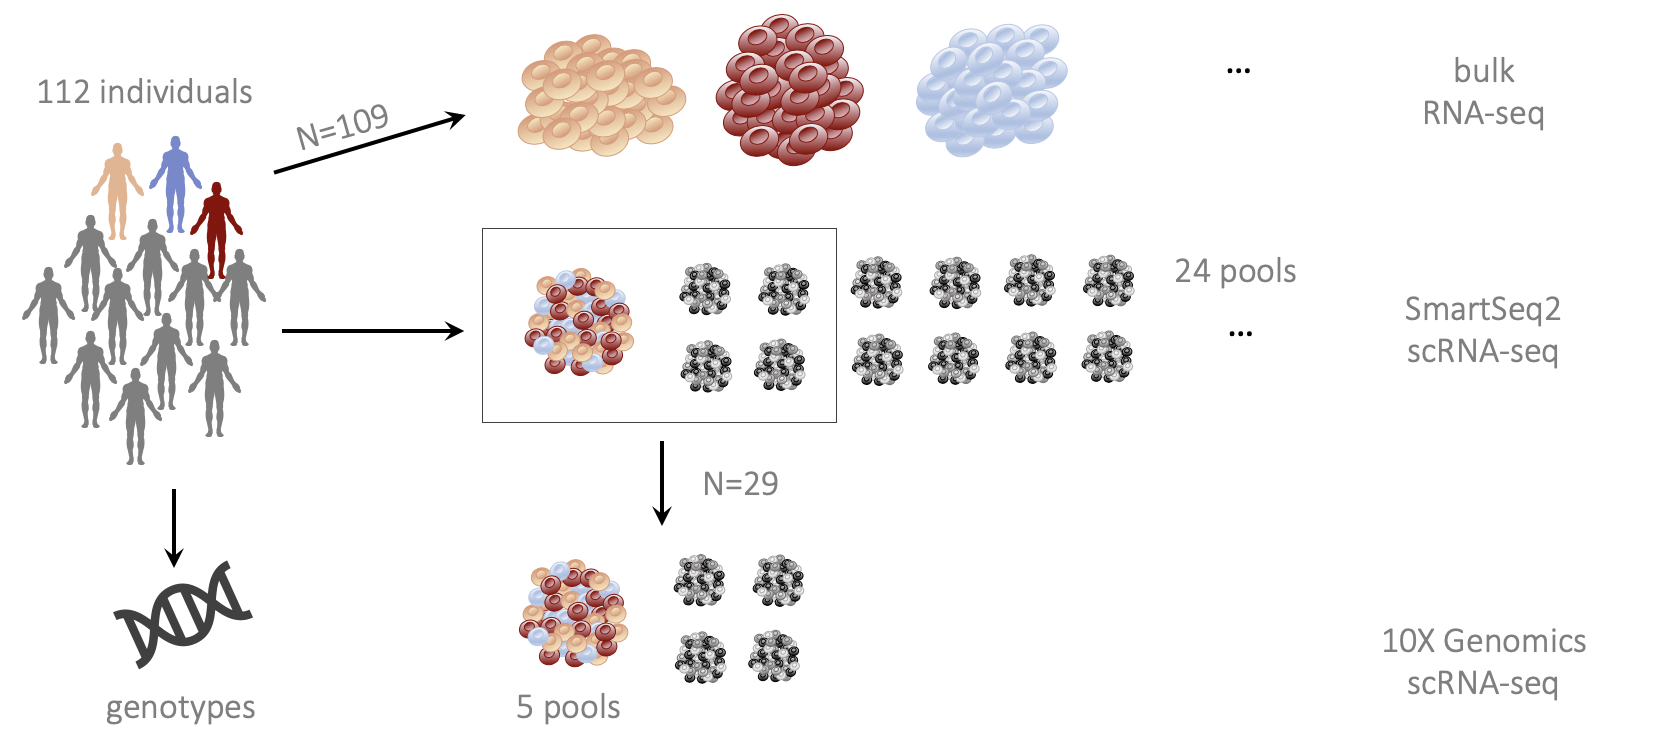
\includegraphics[width=14cm]{Chapter3/Fig/ips_data.png}
\caption[iPSC data]{\textbf{Overview of iPSC data used in this chapter}.\\
We use SmartSeq2 \cite{purcell2007plink} data from 111 \gls{ipsc} lines (from 111 individuals) from \cite{cuomo2020single}, across 24 experimental pools, each containing cells from 4-6 lines (middle).
For 108 of those lines, we have bulk RNA-seq profiles from \cite{mirauta2018population} (top).
Finally, for five of the pools (corresponding to 29 individuals/lines), we also have scRNA-seq data sequenced using the 10X Genomics pipeline \cite{zheng2017massively} (bottom).}
\label{fig:ipsc_data}
\end{figure}

\section{eQTL mapping pipeline}

To map \glspl{eqtl}, I use a pipeline primarily written by Marc Jan Bonder, to which Bogdan Mirauta, Daniel Seaton, Na Cai and myself have also contributed. 
It is a wrapper around LIMIX \cite{lippert2014limix, casale2015efficient}, and it is publicly available at \url{https://github.com/single-cell-genetics/limix_qtl}. \\

For all three eQTL maps (single cell SmartSeq2, bulk, single cell 10X), I used the same exact pipeline and tested the same set of genes (n=10,840).
In particular, I performed \textit{cis} \gls{eqtl} mapping, considering common (minor allele frequency > 5\%), in HWE (p value > 0.001)\footnote{HWE: Hardy-Weinberg equilibrium.}, variants within a \textit{cis}-region spanning 250 kb up- and down-stream of the gene body.
% for \textit{cis} QTL analysis. 
For each gene-SNP pair, the association test was performed using an LMM (\textbf{section
\ref{sec:linear_mixed_models}}):
% 2.3.2}):

\begin{equation}\label{eq:LMM_ipsc_eqtl}
    \mathbf{y} = \sum_i^{P}\alpha_i \mathbf{PC}_i + \mathbf{g}\beta + \mathbf{u} + \boldsymbol{\psi},  
\end{equation}
where 
\begin{itemize}
    \item $\mathbf{y}$ is the $N \times 1$ standardised\footnote{Centered at 0 and scaled to have variance = 1.} expression phenotype vector (details in next section),
    \item the first P=10 PCs calculated on the expression values (matrix with $\mathbf{y}$ as columns, before standardisation) are included as covariates\footnote{This is a common approach to correct for possible batch effects, which usually affect the expression of many genes, and therefore are detectable in the principal components of expression. 
    Moreover, these global effects are orthogonal to the effects of a single variant on the expression of one gene (see \textbf{section 
    % 2.2.4
    \ref{sec:confounders}}).}, and $\alpha_i$ are the corresponding weights,
    \item $\mathbf{g}$ is the $N \times 1$ vector of alleles for each sample at the locus tested (modelled as the number of minor alleles present - 0, 1 or 2), and $\beta$ is the corresponding effect size,
    \item $\mathbf{u}$ is a random effect term used to account for 
    the samples' 
    population structure, 
    % such that: 
    i.e.
    $\mathbf{u} \sim \mathcal{N}(\mathbf{0}, \sigma_g^2\mathbf{K})$, where $\mathbf{K}$ is an $N \times N$ kinship matrix estimated using PLINK \cite{purcell2007plink},
    \item and $\boldsymbol{\psi} \sim \mathcal{N}(\mathbf{0}, \sigma_n^2\mathbf{I})$, where $\mathbf{I}$ is the $N \times N$ identity matrix, is the noise vector.
\end{itemize}

\vspace{1.5mm}

\newpage

% Association tests were performed using a linear mixed model (LMM), accounting for population structure and sample repeat structure (see below) as random effects (using a kinship matrix estimated using PLINK\cite{purcell2007plink}).
% , with no observed confounding between population structure and experimental batch (Supplementary Fig. 24). 
All models were fitted using LIMIX \cite{lippert2014limix, casale2015efficient}. 
The significance was tested using a likelihood ratio test (i.e. $\beta \neq 0$, \textbf{section 
\ref{sec:hypothesis_testing}}).
% 2.2.1}).
In order to adjust for multiple testing (\textbf{section
\ref{sec:multiple_testing}}),
% 2.2.2}), 
we used a permutation scheme, analogous to the approach proposed in Ongen \textit{et al}. \cite{ongen2016fast}. 
Briefly, for each gene, we generated 1,000 permutations of the genotypes while keeping covariates, kinship, and expression values fixed. 
We then adjusted for multiple testing using this empirical null distribution.
To control for multiple testing across genes, we then applied the Storey procedure \cite{storey2003statistical}. 
Genes with significant \glspl{eqtl} were reported at FDR < 10\%.

% \newpage

\section{Single cell eQTL map of iPS cells}
\label{sec:sc_ipsc_eqtl}

Using the method just described, we first tested for associations between common genetic variants and gene expression in \glspl{ipsc} using our SmartSeq2 single cell data.\\

To reproduce bulk-like abundance measurements, we considered a gene's average expression level for each sample, across cells.
In particular, expression level is measured as log2(CPM+1)\footnote{CPM: counts per million, mapped reads are count-scaled by the total number of fragments sequenced per cell, times one million.} using scater \cite{mccarthy2017scater}.
% size factor?
\\

Since we did not use any batch correction method on the single cell expression data \textit{a priori}, we cannot exclude differences across batches.
As internal control we have, for a subset of donors (23/112), data from two (or three, in one case) distinct experimental batches.
We therefore compute average expression levels not for each individual line, but for each line-experiment combination (i.e. cell\_lineA-experiment1, cell\_lineA-experiment2), which enables effective correction for batch-to-batch differences using PCs as covariates (see above and \textbf{section
\ref{sec:confounders}}).
% 2.2.4}). 
% However, to be able to correct for possible batch differences, we considered two different average expression measures, when the same line was assessed in two different experimental batches - individual 1 in experiment A and individual 1 in experiment B are considered as two distinct samples.
% \subsection{Technical considerations}
The linear mixed model described in eq. \eqref{eq:LMM_ipsc_eqtl} can be readily adapted to include the resulting replicate measures from the same line: $N$ will now be not the number of unique lines but that of line-experiment combinations.
Additionally, both the genotype vector $\mathbf{g}$ and the kinship matrix $\mathbf{K}$ need to be adjusted\footnote{i.e. expanded, by duplicating genotype values across pool replicates.}, such that the latter is now in fact accounting at once for the population structure and the repeatedness of the samples tested (\textbf{Fig. \ref{fig:kinship_repeats}}). \\

Using this approach, I identified 1,833 genes with at least one \gls{eqtl} (from hereon `eGenes'), at FDR <10\%, out of 10,840 genes tested (17\%). 

\begin{figure}[h]
\centering
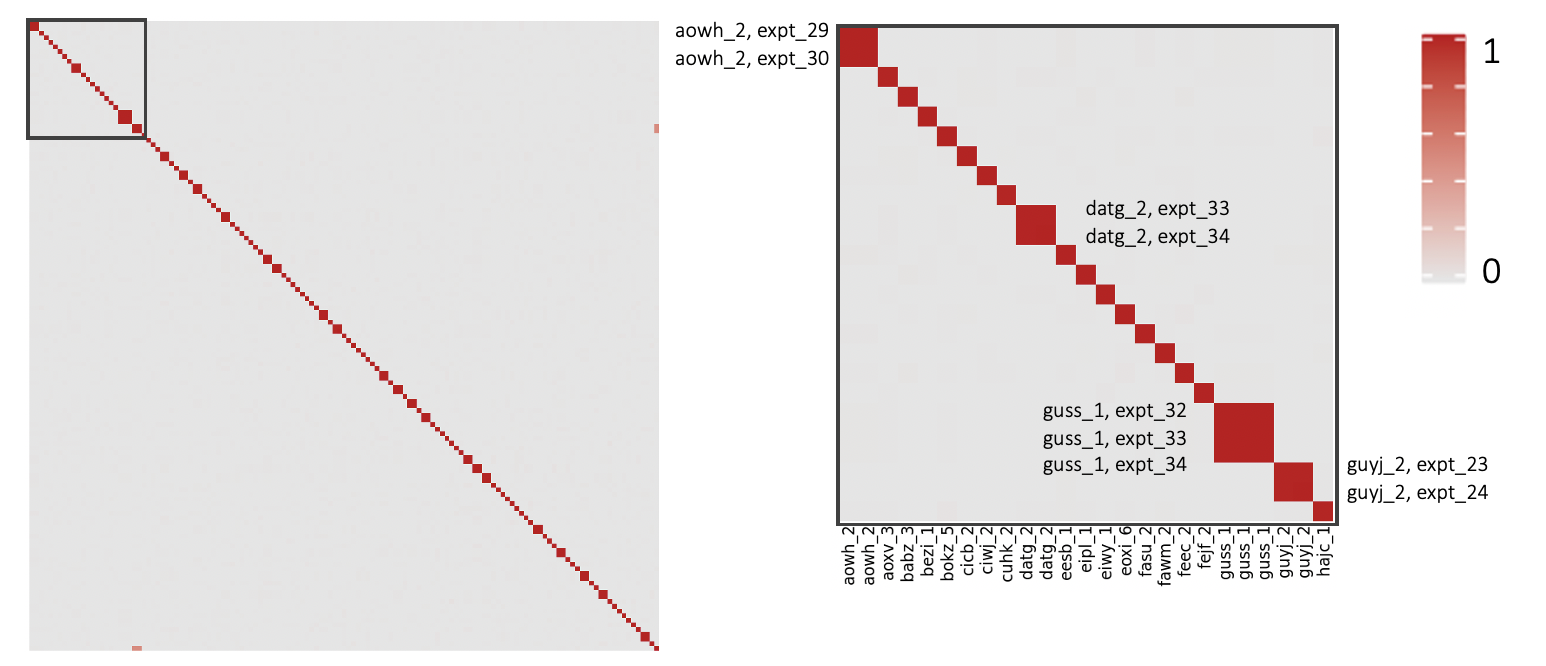
\includegraphics[width=14.5cm]{Chapter3/Fig/kinship_repeatedness.png}
\caption[Kinship for repeated samples]{\textbf{Kinship matrix highlighting repeated structure of samples used}.\\
Heatmap of the kinship matrix used to map \glspl{eqtl} using single cell data.
% Red indicated a maximum degree of relatedness, grey absence of it.
% The binary look of the heatmap suggests that lines used are from essentially unrelated individuals.
% The only pattern of relatedness is present for replicate observations from the same line, across experimental batches.
Replicate observations for a line across experimental batches are genetically identical, which is captured by the kinship (maximum relatedness, red).
Line-to-line relatedness is effectively 0 (grey), indicating unrelated individuals. 
On the right, zoom-in to only consider the first 20 \gls{ipsc} lines, highlighting the repeated samples.}
\label{fig:kinship_repeats}
\end{figure}

% \subsection{Results}

% CPM = readsMappedToGene * 1/totalNumReads * 10$^6$, totalNumReads - total number of mapped reads of a sample, readsMappedToGene - number of reads mapped to a selected gene




% \subsection{LMM}
% Association tests were performed using a linear mixed model (LMM), accounting for population structure and sample repeat structure (see below) as random effects (using a kinship matrix estimated using PLINK\cite{purcell2007plink}).
% % , with no observed confounding between population structure and experimental batch (Supplementary Fig. 24). 


\newpage

\section{Replication of iPSC eQTL using bulk RNA-seq}

For comparison, I performed \textit{cis}-\gls{eqtl} mapping using the matched bulk RNA-seq data.
% considering only the cell lines that had been used to map \gls{ipsc} \glspl{eqtl} from the scRNA-seq data (bulk data was available for 108 donors out of the 112 day0 single cell donors), 
I used the same pipeline (eq. \eqref{eq:LMM_ipsc_eqtl})\footnote{The only difference of course is that there were not multiple replicates from the same line in the bulk RNA-seq data, but the model in eq. \eqref{eq:LMM_ipsc_eqtl} still holds.} 
and tested the same set of genes. 
This yielded 2,908 significant genes at an FDR of 10\%
% (out of 10,736 genes tested, 27\%)
(27\% of genes tested). \\

I found that over 70\% of \glspl{eqtl} identified using scRNA-seq data were replicated in the bulk study, where a single-cell \gls{eqtl} lead variant (top variant per gene) was replicated if it achieved nominal significance (p value < 0.05) and had consistent direction of effect in the full set of results from the bulk \gls{eqtl} analysis (\textbf{Fig. \ref{fig:sc_bulk_egenes}}). \\

On the other hand, only around 50\% of the \gls{eqtl} identified (at FDR < 10\%) using bulk RNA-seq could be replicated
% \footnote{Defined as above: nominal significance (p value < 0.05) and same direction of effect.} 
in our single cell \gls{eqtl} map.
However, when we subsetted to \gls{eqtl} identified using bulk data at a more stringent FDR threshold (1\%), the replication proportion was much larger (76\%), and the more stringent the FDR threshold, the more bulk \gls{eqtl} we could replicate using single cell data (\textbf{Fig. \ref{fig:sc_bulk_egenes}}).
This result suggests that we are able to detect the stronger \gls{eqtl} signals, but lack the power (compared the corresponding test using bulk RNA-seq profiles) to identify smaller effects.
% \\

\begin{figure}[h]
\centering
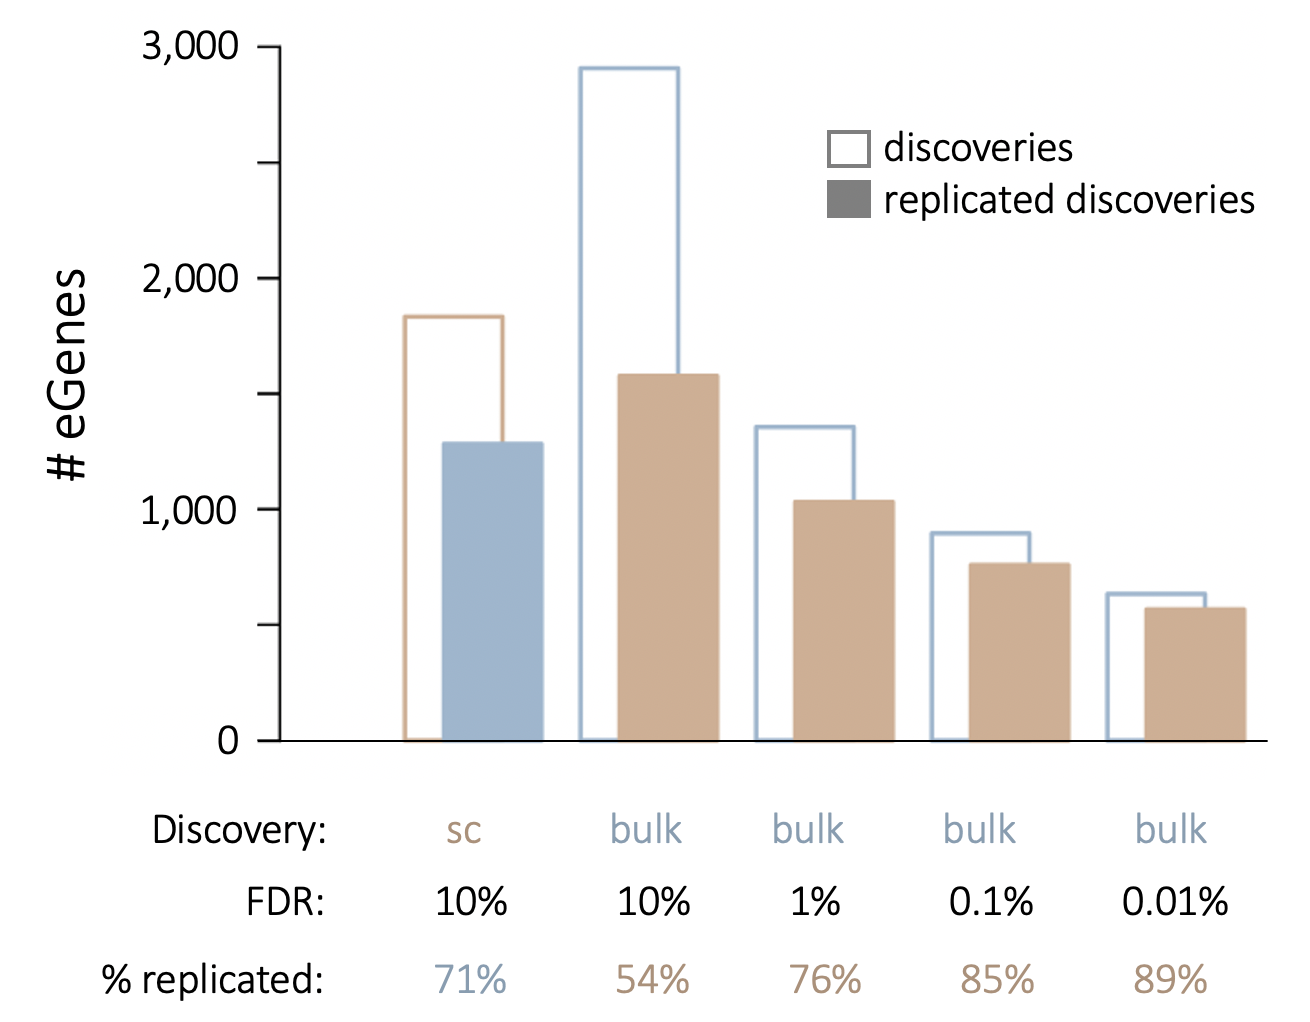
\includegraphics[width=12cm]{Chapter3/Fig/sc_vs_bulk_eqtl.png}
\caption[iPSC eQTL (bulk vs sc)]{\textbf{Replication of iPSC bulk eQTL using single cell data and vice versa}.\\
Replication of \gls{ipsc} \gls{eqtl} discovered with (matched-sample) bulk RNA-seq data using scRNA-seq data, and vice versa.
The total number of eGenes discovered is shown, along with the number of discoveries replicated in the other dataset, at various FDR thresholds. 
% Replication of bulk \gls{eqtl} in single-cell RNA-seq (SmartSeq2, here SS2) on same set of samples increases with significance ($\sim$55\% at FDR 10\%, $\sim$90\% at FDR 0.01\%, 4/112 samples were not present in the bulk RNA sequencing dataset).
sc: single cell.}
\label{fig:sc_bulk_egenes}
\end{figure}

% To compare the \gls{ipsc} \gls{eqtl} maps derived from bulk and single-cell RNA-seq data, we assessed the nominal significance (p value < 0.05) as well as the consistent direction of effect of single-cell \gls{ipsc} \gls{eqtl} lead variants (top variant per gene) in the full set of results from the bulk \gls{ipsc} \gls{eqtl} analysis and vice versa.

% To validate our approach, we also performed \gls{eqtl} mapping using deep bulk RNA-sequencing profiles from the same set of \gls{ipsc} lines (`iPSC bulk'; 10,736 genes tested) generated as part of the \gls{hipsci} project \cite{kilpinen2017common}, yielding consistent \gls{eqtl} ($\sim$70\% replication of lead \gls{eqtl} effects; nominal p value < 0.05).\\ 

\newpage

\section{Replication of iPSC eQTL using 10X data}

Next, to further confirm our \gls{ipsc} \gls{eqtl} map, we performed \gls{eqtl} analysis (eq. \eqref{eq:LMM_ipsc_eqtl}) using scRNA-seq data generated from a subset of 5 experiments (29 lines) using a droplet-based approach (10X Genomics \cite{zheng2017massively}, \textbf{Fig. \ref{fig:ipsc_data}}).\\

Similar to before, we assessed how many bulk-identified \gls{ipsc} \gls{eqtl} could be replicated using 10X samples.
Since this study is fairly underpowered with only 29 samples, we did not consider the opposite analysis, i.e. 10X discoveries replicated in bulk.
We did, however, compare results to an \gls{ipsc} \gls{eqtl} map using the SmartSeq2 data, when sub-setted to the same 5 experiments (and 29 lines). \\

Overall, we observe that replication of bulk \gls{eqtl} using scRNA-seq is reduced when we reduce sample size (for example, at FDR < 10\% replication was 41\% using 29 lines compared to 54\% using all 111 lines in \textbf{Fig. \ref{fig:sc_bulk_egenes}}), but comparable across technologies (SmartSeq2, 10X Genomics), with SmartSeq2 slightly outperforming 10X (\textbf{Fig. \ref{fig:sc_bulk_10x_egenes}}).
% \\

\begin{figure}[h]
% \centering
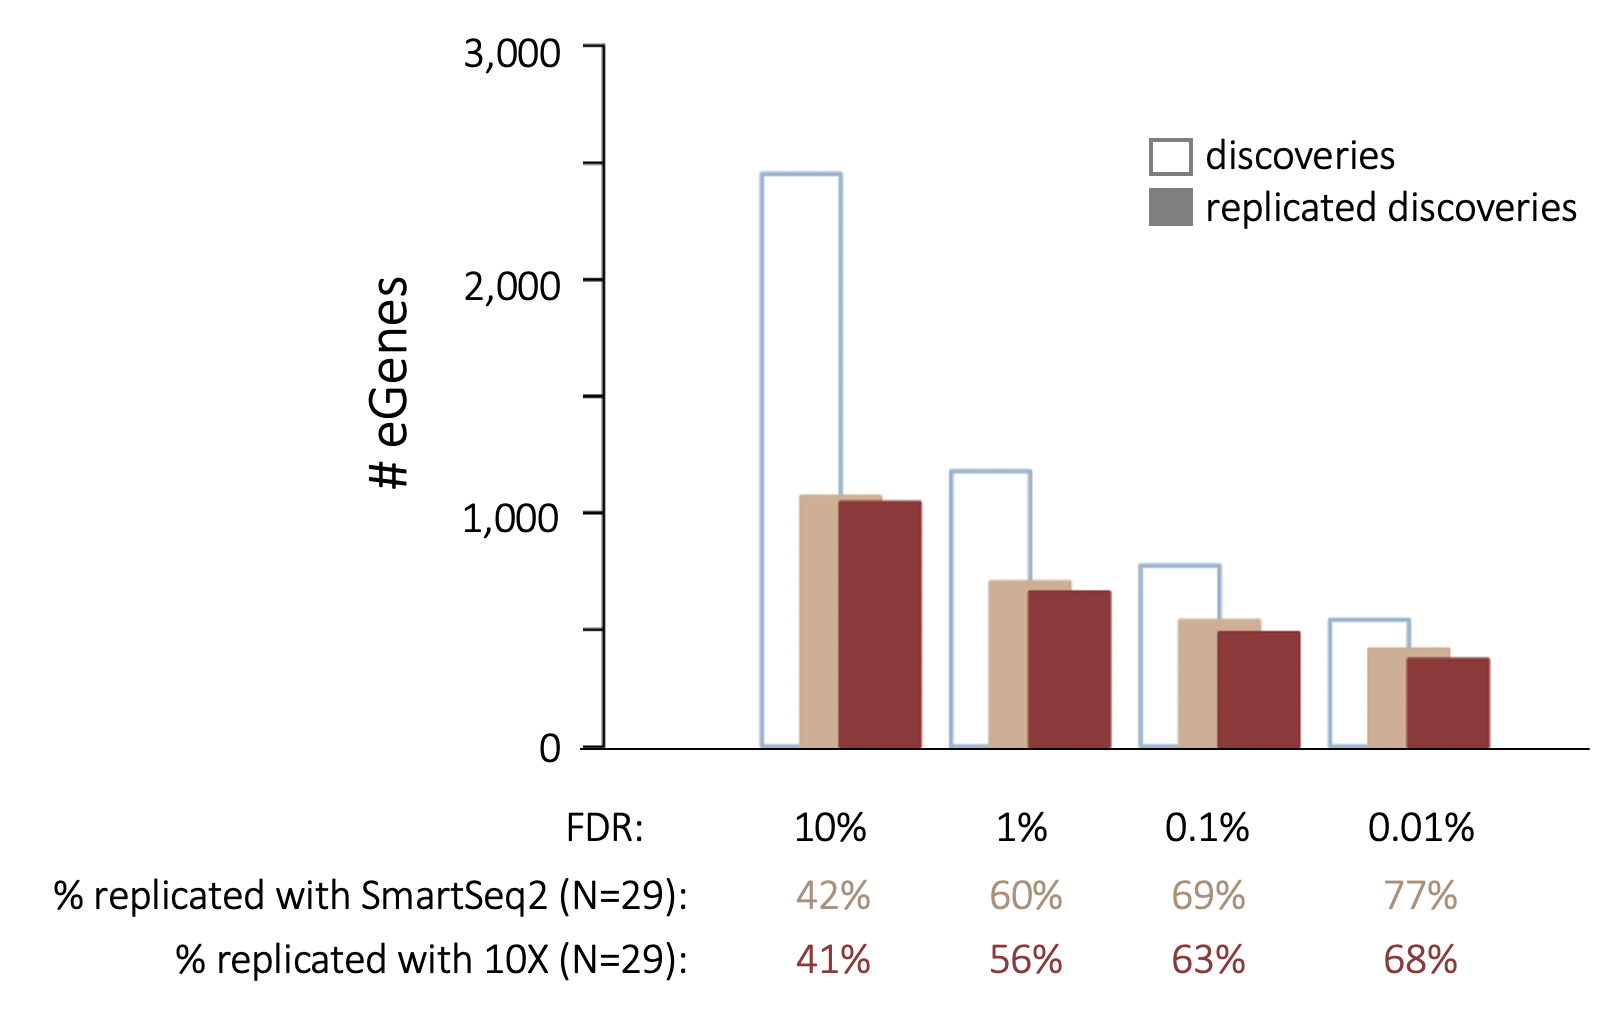
\includegraphics[width=14.5cm]{Chapter3/Fig/sc_vs_bulk_vs_10x.png}
\caption[iPSC bulk eQTL replication]{\textbf{Replication of iPSC bulk \gls{eqtl} using single cell across technologies}.\\
Replication of \gls{ipsc} \gls{eqtl} discovered with bulk RNA-seq (108 samples), using single cell RNA-seq data from a common set of 29 samples (SmartSeq2 in sand, 10X Genomics in red). 
The total number of bulk eGenes discovered is shown, along with the number of discoveries replicated using single cell profiles, at different FDR thresholds. 
As before, replication was defined as nominal significance, at p value < 0.05, and same direction of effect.}
\label{fig:sc_bulk_10x_egenes}
\end{figure}

\newpage

Additionally, we found good agreement in terms of effect sizes between the \gls{eqtl} maps obtained using the two different single cell technologies, highlighting the robustness of the approach (\textbf{Fig. \ref{fig:sc_eqtl_technologies}}). \\

\begin{figure}[h]
\centering
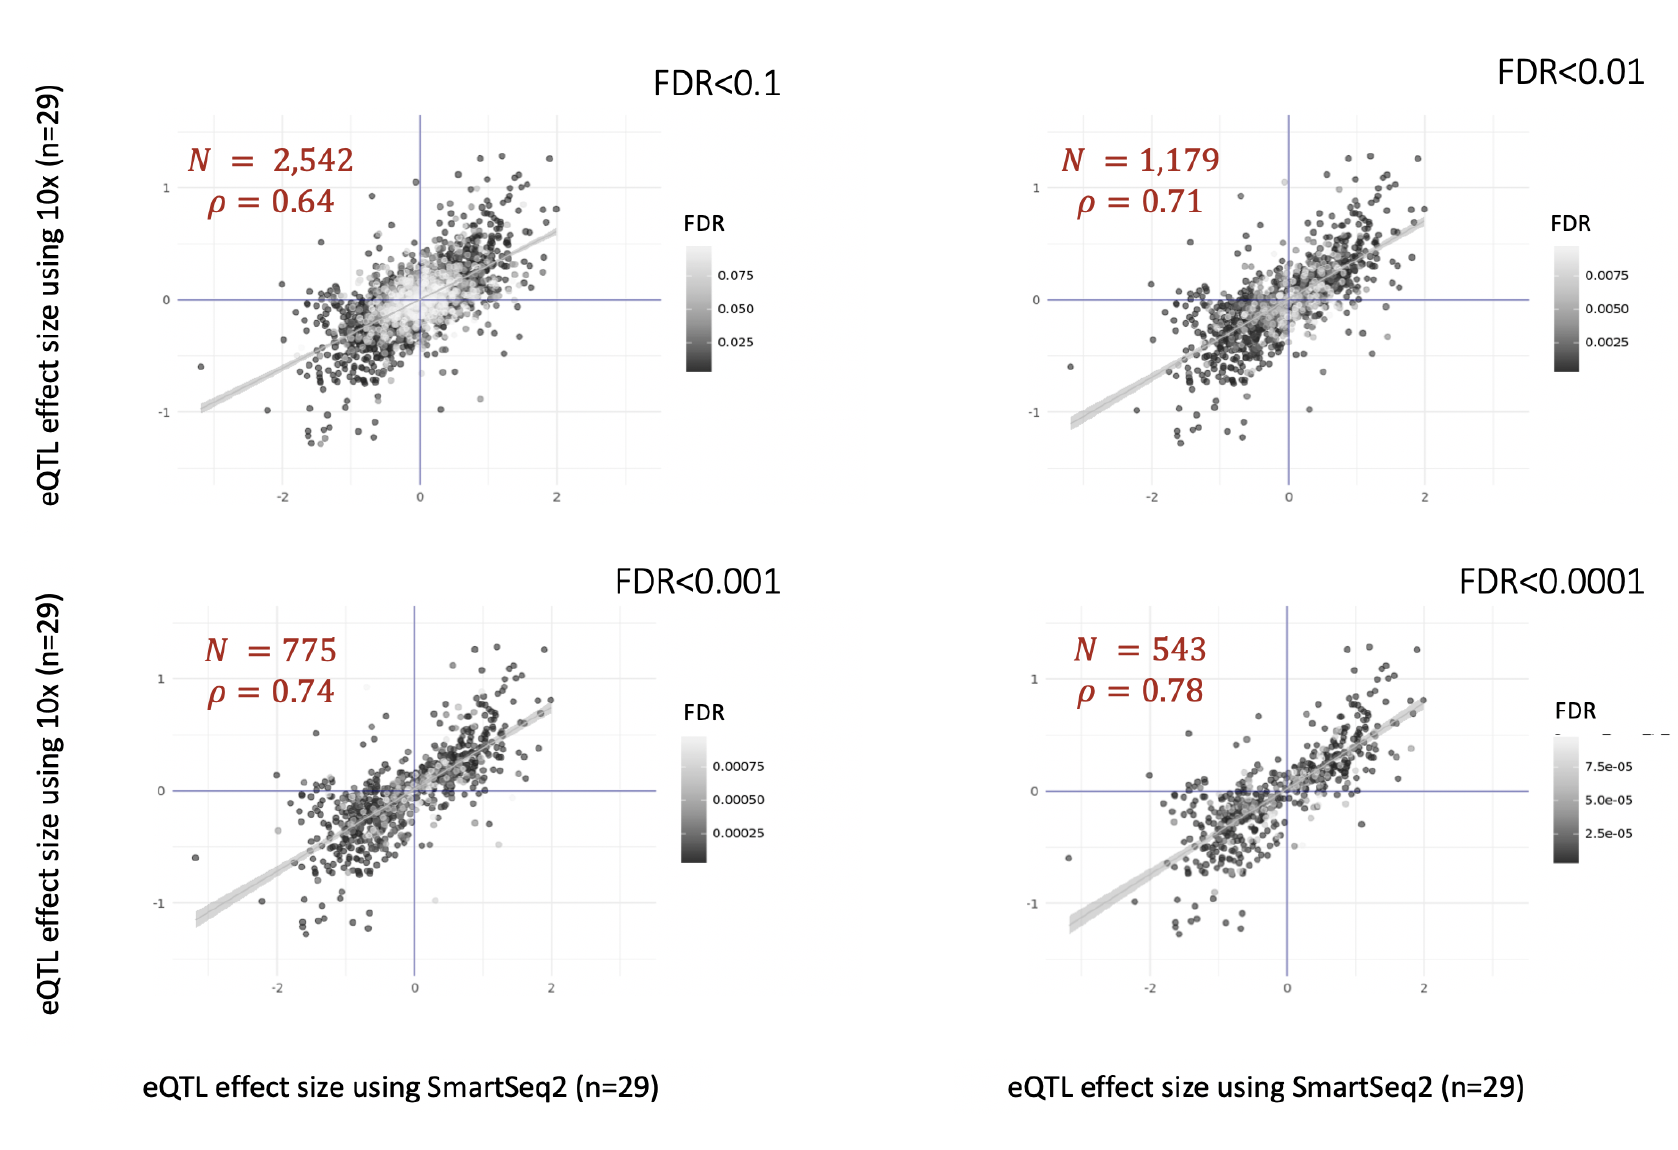
\includegraphics[width=15cm]{Chapter3/Fig/beta_comparison_ss2_vs_10x.png}
\caption[iPSC sc-eQTL replication across technologies]{\textbf{Effect size agreement between single cell technologies.}\\
Scatter plots of \gls{eqtl} effect sizes obtained when testing association of \gls{ipsc} \gls{eqtl} discovered using bulk RNA-sequencing (108 cell lines), using SmartSeq2 (\cite{picelli2013smart} x axis) and 10X Genomics (\cite{zheng2017massively} y axis) on cells from 5 experimental batches (experiments 31, 40, 41, 43, 44; 29 cell lines in total). 
The number of \gls{eqtl} examined and the correlation between effect sizes is indicated when we consider bulk \gls{ipsc} \gls{eqtl} discoveries at four different FDR thresholds (0.1, 0.01, 0.001, 0.0001).}
\label{fig:sc_eqtl_technologies}
\end{figure}

% As we acknowledge
Since the vast majority of scRNA-seq datasets presented recently use droplet-based (rather than plate-based) technology, as it allows, as we have seen (\textbf{page \pageref{fig:scrnaseq_plate_vs_droplet}}), the assessment of a much larger number of cells in a single experiment, it is important to show that this approach would work for such datasets as well. 
Whilst in this case we had data from too few individuals to make a very strong argument, the good concordance of results between 10X and SmartSeq2 suggests that this approach would work well for all single cell RNA-seq datasets, across technologies.

\clearpage

\section{Preliminary steps towards a best-practice pipeline}
\label{sec:best_practice}

The results presented so far are included in Cuomo \textit{et al}. \cite{cuomo2020single}, the other results of which I discuss in detail in the next chapter (\textbf{Chapter 
% 4
\ref{chapter4}}). \\

More recently, in collaboration with Marc Jan Bonder and Giordano Alvari from the Stegle group, I have worked on a best-practice pipeline which extends on the work presented so far, by testing the effect of different parameters of the model, to optimise yield of single cell eQTL mapping.
In particular, using the same iPSC data described so far (\textbf{Fig. \ref{fig:ipsc_data}}), we systematically compared results when mapping eQTL i) using various aggregation strategies to obtain `pseudo-bulk' expression levels to use as phenotypes in the model, and ii) varying the type and number of `global expression effect' covariates (see \textbf{section
\ref{sec:confounders}})
% 2.2.4}) 
that are included in the model.
% Finally, we evaluated normalisation strategies for the expression profiles used as phenotype.

\subsection{Overview of the iPSC data used}

As I have mentioned, we broadly use the same iPSC data as before, i.e. scRNA-seq from \cite{cuomo2020single} and (matched) bulk RNA-seq from the HipSci resource.
% rephrase this sentence
% However, we adopted a rather conservative approach with respect to the data included, to optimise this comparison. \\
However, we implemented some changes, to increase our confidence in this comparison. 
% \\
First, to make the data most comparable between the scRNA-seq data and the bulk RNA-seq data, we re-quantified single cell expression at the gene level using the `featureCounts' tool \cite{liao2014featurecounts}, as was done for the bulk RNA-seq data (rather than relying on the quantification using the pseudo-aligner salmon \cite{patro2017salmon}, which was used to obtain the results described above and all results in \textbf{Chapter \ref{chapter4}}).
% , which would have been inconsistent across technologies). 
\\

% Briefly, adapters were trimmed from reads using Trim Galore!, using default settings. 
% Trimmed reads were mapped to the human reference genome build 37 using STAR (version: 020201) in two-pass alignment mode, using the defaults proposed by the ENCODE consortium (STAR manual). 
% Gene-level RNA expression was quantified from the STAR alignments using featureCounts (v1.6.0), which was applied to the primary alignments using the `-B' and `-C' options in stranded mode if applicable, using the Ensembl 75 GTF file. \\

Additionally, to remove further possible confounding effects, a small group of lines from monogenic diabetes donors were excluded, as well as four lines which were slight outliers in the genotype space (\textbf{Fig. \ref{suppl_fig:kinship_pcs}}).
% excluded one line slightly off ethnicty-wise, other? i.e. at least X cells? (n=88?)
In total, we map single cell eQTL for 88 cell lines (from 88 donors).
As a cell QC step, we calculated the average correlation of each cell with all other cells.
Then, for each sequencing run, we calculated the median of the resulting cell-correlation values.
If a run had median cell-correlation < 0.7, all cells from the run were discarded (\textbf{Fig. \ref{fig:sc_eqtl_autocorrelation}}, panel a).
In a second step, cell-cell correlations were calculated again, between cells from the remaining runs only.
% All cells that had average correlation < 0.5 after this second step were also discarded (\textbf{Fig. \ref{fig:sc_eqtl_autocorrelation}}). 
This time, we considered line-run combinations, and discarded all combinations that had median cell-correlation < 0.5 (\textbf{Fig. \ref{fig:sc_eqtl_autocorrelation}}, panel b). \\

\begin{figure}[h]
\centering
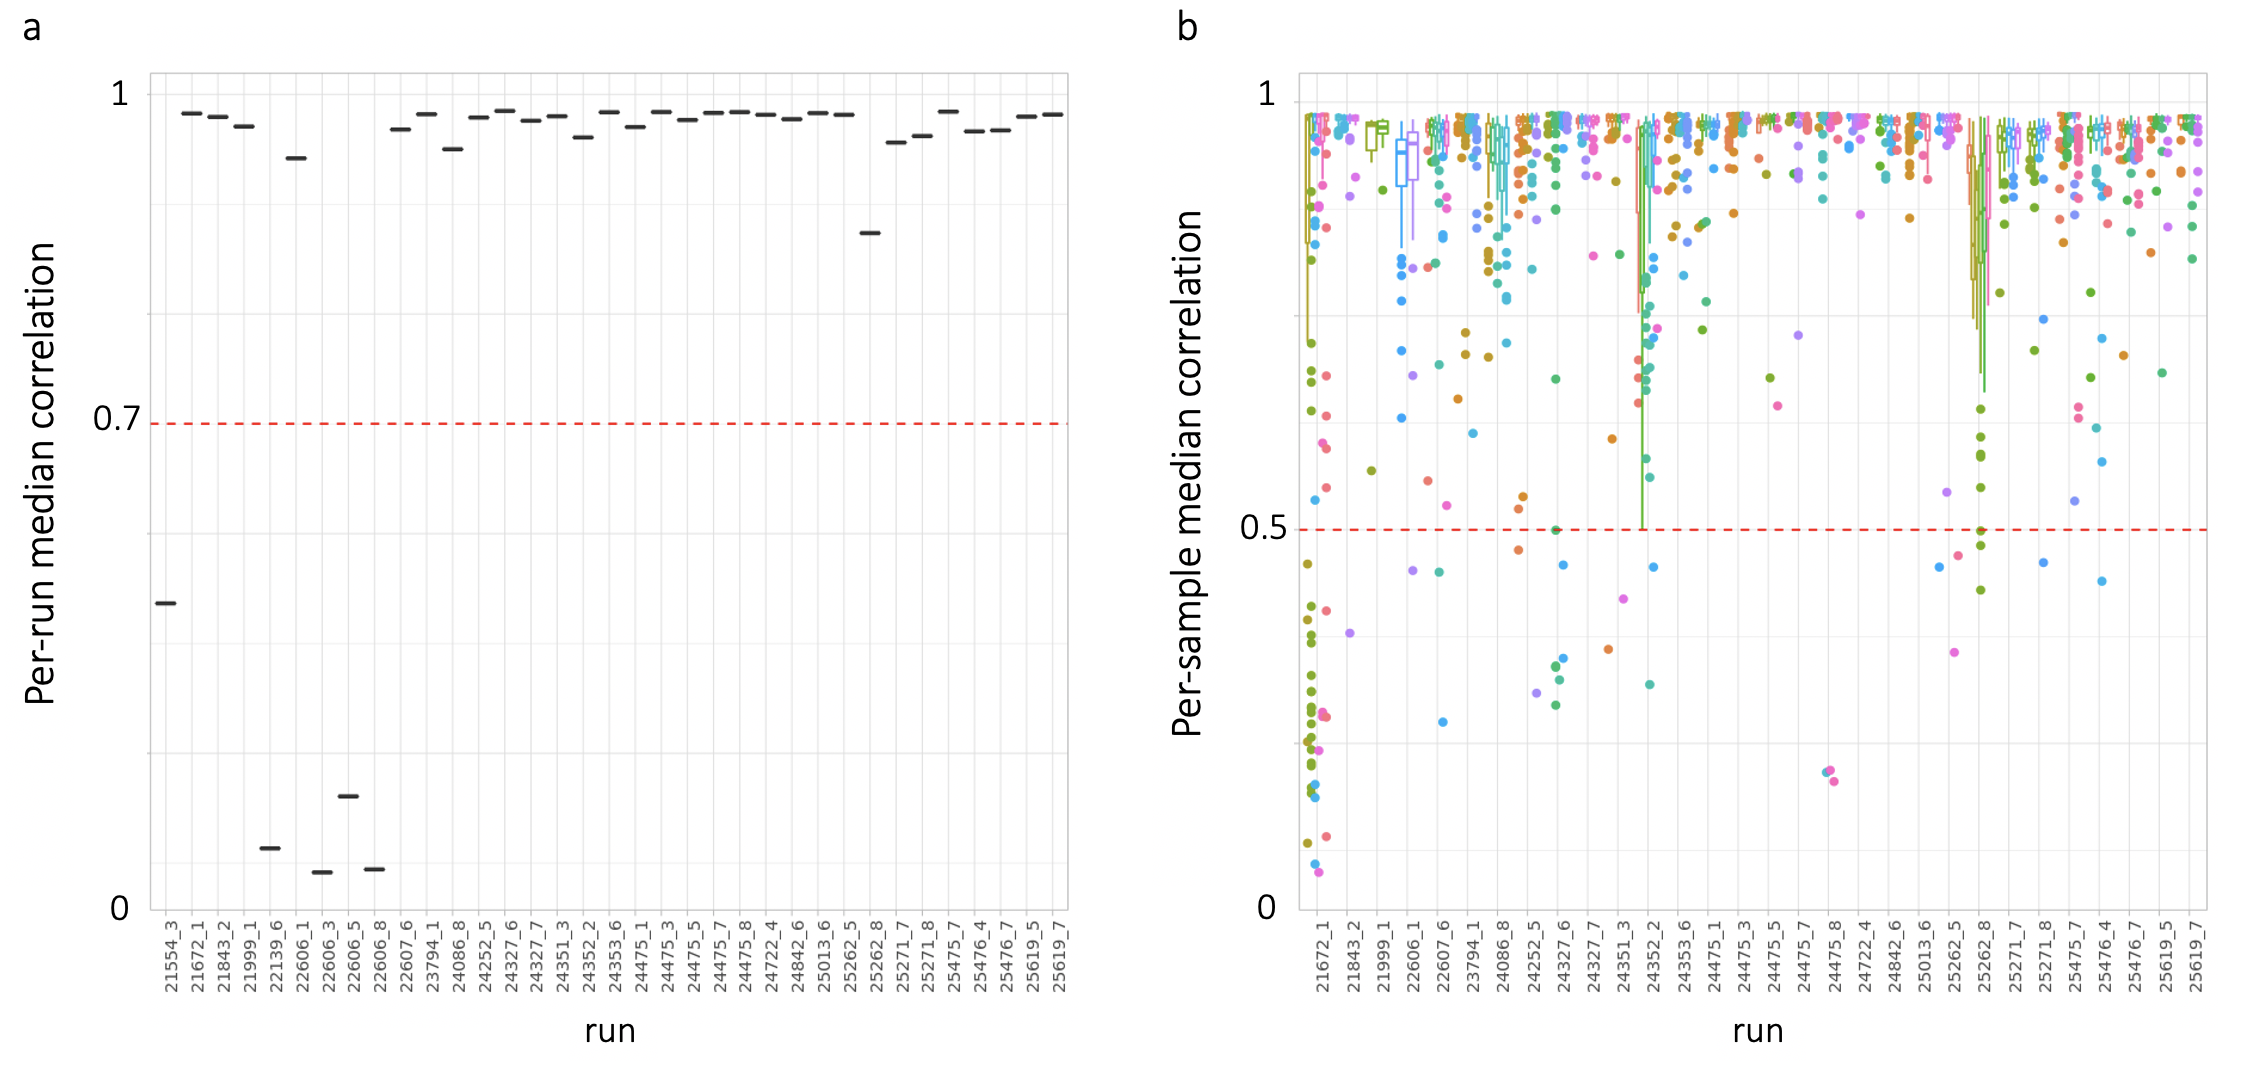
\includegraphics[width=15cm]{Chapter3/Fig/sc_eqtl_cell_QC.png}
\caption[Correlation-based cell QC]{\textbf{Correlation-based cell QC}\\
(a) Median cell-correlation calculated per run.
Runs with median cell-correlation < 0.7 were discarded.
(b) For the remaining runs, donor-run (i.e. sample) level median cell-correlations were calculated, and samples with median cell-correlation < 0.5 were discarded.}
\label{fig:sc_eqtl_autocorrelation}
\end{figure}

\newpage

Moreover, in order to compare eQTL results across genes at different expression levels, we chose to be more lenient on the criteria for gene inclusion.
% , such that we could test up to 50,425 genes in total. 
Indeed, we considered all variable genes as obtained by ranking all genes (n=50,425) by their squared coefficient of variation ($CV^2$)\footnote{$CV^2=\sigma^2/\mu^2$.} across all cells, and selecting the upper two quartiles.
As a result, 20,545 genes were included in the analysis. 
On the other hand, to reduce the multiple testing burden, we only tested SNPs with MAF >10\% and within a smaller window around the gene (100kb on either side of the gene body).

\subsubsection{Comparison partners}

Finally, we compared the resulting single cell eQTL maps with results obtained using bulk RNA-seq both limited to the same set of samples (n=88, `matched bulk'), and using all samples that were available at the time (n=810 HipSci lines from 527 unique donors, `bulk'). 

% % In order to produce bulk-like results, two main approaches can be used.

% % Under the assumption that we are looking at a single cell type, we can i) aggregate counts across all cells from an individual (e.g. taking the average expression value) and generate a `pseudo-bulk' measure, and then run the test exactly as if it were bulk; or ii) use full single cell expression, without aggregating.

% % % In this chapter, we introduce the two datasets that we will use throughout the thesis, setting the scene for all other chapters. 
% % % These are among the very first datasets of their kind, assessing single cell gene expression profiles for hundreds of genetically diverse individuals, allowing to interrogate the effect of common genetic variation on transcriptional variability.
% % % Previously, most \gls{eqtl} mapping studies in humans were performed using bulk RNA-sequencing, and most scRNA-seq studies were performed in a handful of individuals only, or in model organisms (often also limited to a few strains).
% % % Notably, one study performed \gls{eqtl} mapping using scRNA-seq \cite{van2018single} recently in blood cells. 
% % % However, this data is limited to 45 individuals and to a single time point, lacking the differentiation axis of our studies.

% % % \subsection{Datasets}

% % % \begin{itemize}
% % %     \item iPS data
% % %     \item simulated data
% % % \end{itemize}

% % \subsection{Data}

% % We use iPS data from \cite{cuomo2020single} - day0 only, etc

% % Smartseq2 \cite{picelli2013smart} data from 10,000 (get exact number) cells from 112 unique unrelated donors, across YY differentiation experiments. 

\newpage

\subsection{Aggregation strategies}

% Add something about sum vs mean, what's more obvious, bla bla normalisation + batch effects and whether to aggregate by donor or not..
% Introduce this. 
% Also repeat this is after cell type identification and QC.\\

% Pseudobulk approach.
As a first step, we investigated which aggregation method (aimed at summarising single cell values to a `pseudobulk' level) resulted in the most power to identify single cell \gls{eqtl}.

To do so, we tested the following approaches:

\begin{itemize}
    \item \textbf{Mean}: average expression across cells from each donor and sequencing run\footnote{This is very similar to the approach used in the first part of this chapter, i.e. using the same principle of accounting for batches.
    The difference is that this is done at an even deeper level of batch, i.e. cells from the same experimental pool were sometimes sequenced in more than one run.},
    \item \textbf{Median}: median expression across cells from each donor and sequencing run,
    \item \textbf{Sum}: summed expression across cells from each donor and sequencing run,
    \item \textbf{Total mean}: average expression across all cells from each donor, aggregated across sequencing runs, and finally
    \item \textbf{Total sum}: similar to the total mean, but summing reads instead.
\end{itemize}

% \newpage

For the first three methods, aggregation is done not only at the donor level but also for each individual sequencing run (i.e. all iPS cells from a given donor in a single sequencing run), to account for possible batch effects (see \textbf{page \pageref{sec:sc_ipsc_eqtl}}).
% This is done in an attempt to account for batch effects (needs explaining).
For what we call `total' sum and mean, on the other hand, aggregation (i.e. sum or mean) is done at the donor level only, to maximise the numbers of cells per donor.
In all cases (i.e. using any of the aggregation methods) aggregated expression values were only calculated for samples (i.e. donors or donor-run combinations) with at least 5 cells.

\subsection{Normalisation strategies}

Importantly, normalisation of the scRNA-seq data was performed in different ways depending on the aggregation method used.
For mean (including total mean) and median aggregation of expression data, we performed single cell-level normalisation using two alternative methods, i) scran/scater \cite{mccarthy2017scater} size factor normalisation and ii) baynorm \cite{tang2020baynorm}.
% Briefly, log2(cpm+1) using size factors..
The mean and the median were then calculated on the resulting normalised (logged) counts (\textbf{Fig. \ref{fig:sc_qtl_workflow}}). \\

On the other hand, summed count values (both sum and total sum) were obtained directly from the un-normalised data.
Normalisation was then applied on the resulting pseudo-bulk counts, using methods typically used for bulk RNA-seq data.
In particular, we perform (logged) CPM normalisation using edgeR \cite{robinson2010edger}, accounting for library size (\textbf{Fig. \ref{fig:sc_qtl_workflow}}).

\begin{figure}[h]
\centering
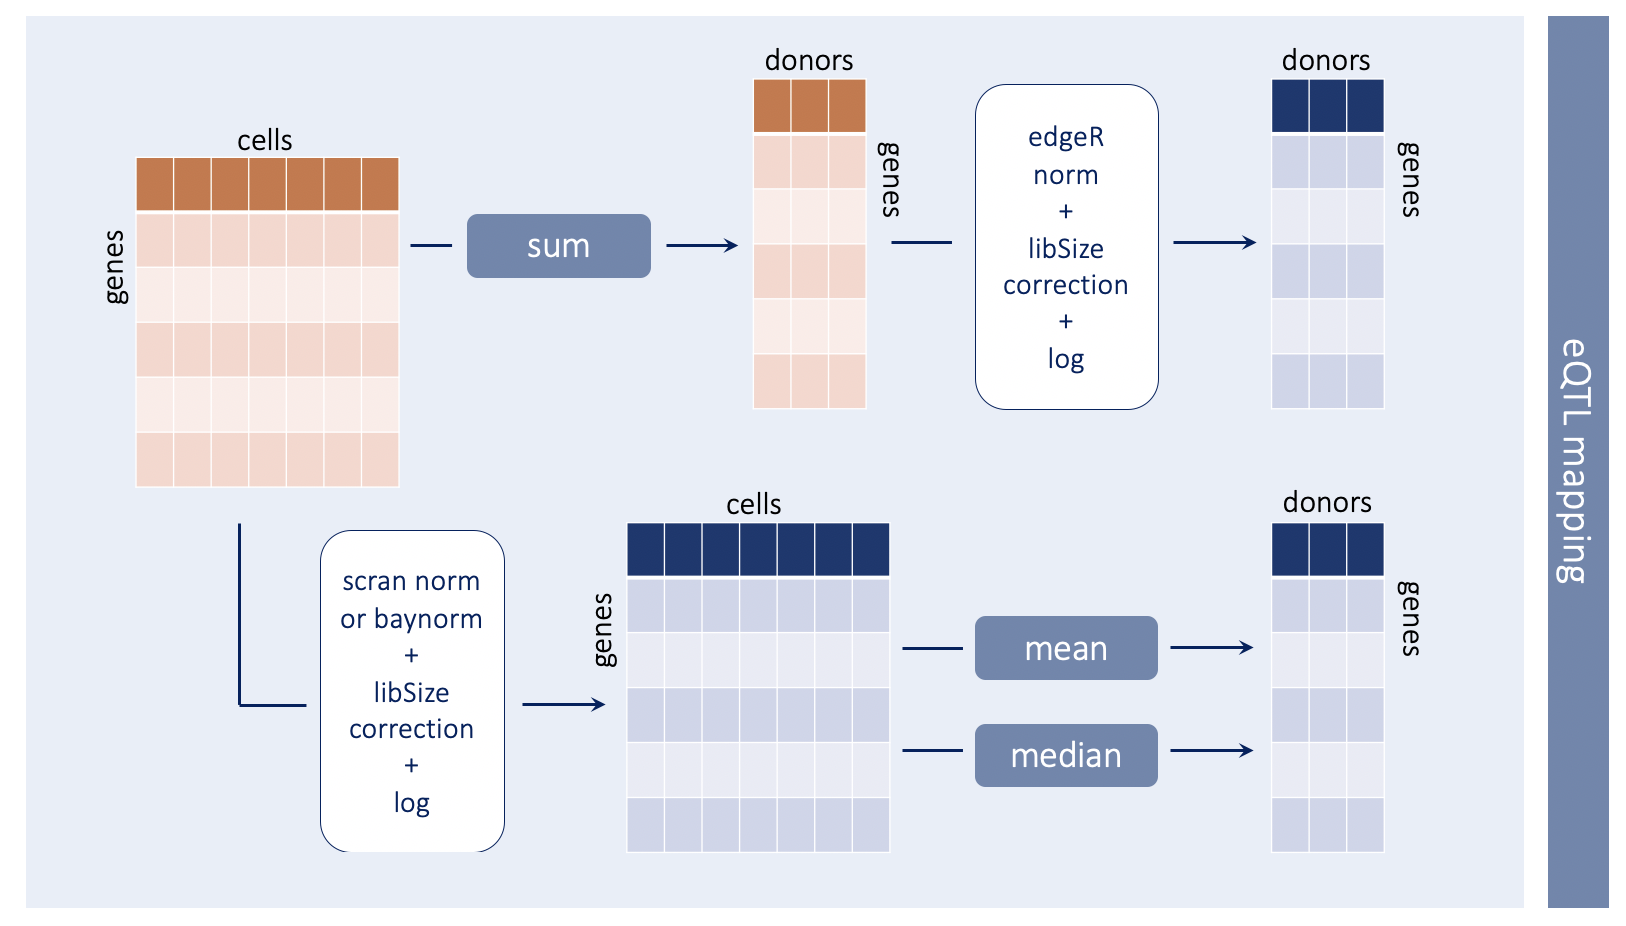
\includegraphics[width=16cm]{Chapter3/Fig/sc_qtl_workflow_no1_2_steps.png}
\caption[sc-eQTL workflow]{\textbf{sc-eQTL workflow}.\\
Different approaches tested to perform \gls{eqtl} mapping using scRNA-seq profiles.
% After processing and QC, and after a homogeneous cell population has been identified (1), and checking across samples correlation i.e. if very low across all genes, may be the wring cell type (2), one count matrix (cells x genes). 
Starting from one gene $\times$ cell count matrix, counts were aggregated per sample (i.e. donor, or donor-run combination), either by summing the data first at sample-level and then normalising using methods designed for bulk RNA-seq (i.e. edgeR \cite{robinson2010edger}) or by first normalising the single cell counts (using scran/scater \cite{mccarthy2017scater} or baynorm \cite{tang2020baynorm}) and then calculating the mean or the median at the sample-level. }
\label{fig:sc_qtl_workflow}
\end{figure}

\subsection{Phenotype transformation}

Linear (mixed) models assume normality of the phenotype vector $\mathbf{y}$ (\textbf{Chapter
\ref{chapter2}}).
% 2}).
However, when using gene expression, we are in the presence of count data.
By log-transforming (log2) and normalising (previous section) such counts, the model-fit is improved, yet this approach still remains sub-optimal (see \textbf{section \ref{sec:non_gaussian}}). \\

In addition, two commonly-used phenotype transformations include standardising each phenotype vector (as I have done before) or quantile-normalising it, i.e. ranking the values and then making the data fit to a Gaussian distribution, forcibly.
Here, we chose the latter strategy, which is more conservative, as it ensures a better fit to the (Gaussian) model.
This approach often results in slightly reduced power but it is more robust, thus better suited for this comparison.

\subsection{Comparing sc-eQTL results across aggregation approaches}

Next, the (normalised and `gaussianised') aggregated expression values resulting from each of the methods described were used to map eQTL.
For this comparison, the first 20 principal components were calculated from each of the aggregated matrices and included in the model as covariates (as before, from eq. \eqref{eq:LMM_ipsc_eqtl}, P = 20).
% Finally, variable genes were obtained by ranking all genes by their squared coefficient of variation ($CV^2$)\footnote{$CV^2=\sigma^2/\mu^2$.} across all cells, and selecting the upper two quartiles (20,545 genes), which were included in the analysis. 
% As mentioned, the aggregated expression values for each of these genes were quantile-normalised and plugged into the pipeline (eq. \eqref{eq:LMM_ipsc_eqtl}), one at a time. 
\\

% \clearpage

\textbf{Table \ref{tab:egenes}} summarises the results across the aggregation methods tested, when restricting the results to the set of 13,167 genes that were tested in each of the eQTL maps.
The comparison is first of all in terms of yield, i.e. number of eGenes identified using each of the methods.
Next, we assess the degree of replication of the discoveries in the set of results obtained using bulk RNA-seq, both using matched samples only, and using all samples.\\

% We observe that the method that performs best is the mean, both in terms of discoveries and consistency with bulk (Table \ref{tab:egenes}).\\

% Results not on common genes, using Giordano's selection:

% \begin{table}[h]
%     \centering
%     \begin{tabular}{c|c c c c c}
%     & \# eGenes & genes tested & \% significant & \% matched bulk  & \% bulk   \\
%     \hline
%     mean         & 2,081 & 20,545 & 10.1\% & 58\% & 71\% \\
%     total mean   & 1,363 & 19,877 & 6.9\% & 66\% & 76\% \\
%     median       & 1,530 & 13,567 & 11.3\% & 48\% & 61\% \\
%     sum          & 1,598 & 20,545 & 7.8\% & 65\% & 75\% \\
%     total sum    & 1,291 & 20,545 & 6.3\% & 66\% & 76\% \\
%     matched bulk & 1,557 & 20,336 & 7.7\% &  - & 97\% \\
%     bulk         & 8,751 & 20,541 & 43\% & - & - \\
%     \end{tabular}
% \end{table}

% Results not on common genes, using Anna's selection:

% \begin{table}[h]
%     \centering
%     \begin{tabular}{c|c c c c c}
%     & \# eGenes & genes tested & \% significant & \% matched bulk  & \% bulk   \\
%     \hline
%     mean         & 1,557 & 10,767 & 14.5\% & 53\% & 70\% \\
%     total mean   & 1,021 & 10,408 & 9.8\% & 62\% & 75\% \\
%     median       & 1,158 & 10,227 & 11.3\% & 53\% & 67\% \\
%     sum          & 1,226 & 10,768 & 11.4\% & 61\% & 74\% \\
%     total sum    & 944 & 10,767 & 8.7\% & 64\% & 78\% \\
%     matched bulk & 790 & 10,766 & 6.3\% &  - & 98\% \\
%     bulk         & 5,093 & 10,772 & 47\% & - & - \\
%     \end{tabular}
% \end{table}

% \newpage

% Common genes (mean, totmean, median, sum, totsum): 13,177,
% including (matched) bulk too: 13,167.

% In Giordano's selection: 13,167.

% In Anna's selection: 9,886.


\begin{table}[h]
    \centering
    \begin{tabular}{c|c c c c c}
    & \# eGenes & genes tested & 
    \% genes tested & 
    % \multicolumn{1}{>{\centering}m{2cm}}{\% genes tested} &
    \multicolumn{1}{>{\centering}m{2.3cm}}{\% replicated in matched bulk} & \multicolumn{1}{>{\centering}m{2.22cm}}{\% replicated in bulk} \\
    % & & & & \% replicated & \% replicated \\
    % & \# eGenes & genes tested & \% genes tested &  matched bulk & bulk \\
    %  \\
    \hline
    mean         &  1,831 & 13,167 & 13.9\% & 66\% & 76\% \\
    total mean   &  1,309 & 13,167 &  9.9\% & 73\% & 81\% \\
    median       &  1,486 & 13,167 & 11.3\% & 55\% & 66\% \\
    sum          &  1,434 & 13,167 & 10.9\% & 70\% & 81\% \\
    total sum    &  1,153 & 13,167 &  8.8\% & 73\% & 82\% \\
    matched bulk &  2,683 & 13,167 & 20.4\% & - & 95\% \\
    bulk         &  9,983 & 13,167 & 75.8\% & - & - \\
    \end{tabular}
    \caption[Aggregation method comparison]{\textbf{Aggregation method comparison.}\\
    For various aggregation methods (rows), and using 20 PCs as covariates, indicated are the total number of eGenes, the percentage of eGenes out of the genes tested (13,167), the percentage of eGenes for which the lead eQTL is replicated when mapping eQTL using bulk RNA-seq with only matched samples (n=88, `matched bulk'), and using all samples (810 lines, 527 donors, `bulk').
    Discoveries using bulk were also added, for reference (last two rows).}
    \label{tab:egenes}
\end{table}



% % The results presented in Table \ref{tab:egenes} are when testing all 20,545 genes (as described above).
% When considering only the 10,408 genes tested above (and presented in \cite{cuomo2020single} and in Chapter 4), the results were equivalent, where we note that yield and bulk replication both are relatively higher when we only consider genes expressed in at least xx cells (Table \ref{tab:egenes_annas_selection}).

% \begin{table}[h]
%     \centering
%     \begin{tabular}{c|c c c c }
%     & \# eGenes & \% genes tested & \% matched bulk  & \% bulk   \\
%     \hline
%     mean         & 1,381 & 13.3\% & \% & \% \\
%     total mean   & 853 & 8.2\% & \% & \% \\
%     median       & 1,106* & 11.2\%* & \% & \% \\
%     sum          & 1,045 & 10.0\% & \% & \% \\
%     total sum    & 797 & 7.7\% & \% & \% \\
%     matched bulk &  & \% & - & \% \\
%     bulk         &  & \% & - & - \\
%     \end{tabular}
%     \caption[Aggregation method comparison, genes from Cuomo \textit{et al.} only]{Same as Table \ref{tab:egenes},  but when only testing the genes selected previously (and assessable in each of these maps, n=10,408 genes).
%     *median testing only 9,886 genes.}
%     \label{tab:egenes_annas_selection}
% \end{table}

These results indicate that considering the mean as the aggregation method is the optimal approach, resulting by far in the most eGenes identified (\textbf{Table \ref{tab:egenes}}).
In terms of replication of bulk results (measured as nominal significance and same direction of effects), the mean results are comparable with the sum, total sum, and total mean, whereas the median, which performed quite well in terms of yield, had substantially fewer of its identified eQTL replicated using bulk. 
Here we note that, although in terms of percentage total mean and total sum outperform the mean, since the number of eGenes is higher, the mean is also the method that identifies the most eGenes replicated in bulk (1,397 vs 1,155 for the second best, the sum). \\

We speculate that whilst the sum would perhaps be the most obvious approach to reproduce bulk-like measurements, the mean might perform better because of the normalisation used.
Indeed, the normalisation at the cell-level may better balance the differences in read counts across cells prior to the aggregation at individual-level. 
Next, we also tested an alternative single cell normalisation approach, baynorm \cite{tang2020baynorm}, and mapped eQTL using the mean aggregation method, finding that the results were virtually indistinguishable (1,834 eGenes vs 1,831, and Pearson's correlation between both p values and effect sizes: R=1, p value < 2.2$\times 10^{-16}$, \textbf{Fig. \ref{suppl_fig:scran_vs_baynorm}}). \\

Reassuringly, we broadly replicated the key results found in the first part of this chapter, confirming that eQTL maps using bulk RNA-seq are better powered that those using single cells, at identical sample size.
Additionally, mean and sum (i.e. aggregating at donor and batch) outperformed total mean and total sum (\textbf{Table \ref{tab:egenes}}), re-iterating the importance of considering replicated experimental designs for eQTL studies.

% add here maybe ROC curve etc

% \clearpage

\subsection{Comparing results using different expression covariates}

% Expression covariates PCs, PEER established (add references, e.g. GTEx..)

As a second comparison, we varied the type and number of expression covariates included in the model to account for global expression variation (see \textbf{section 
\ref{sec:confounders}}).
% 2.2.4}).
Since the mean outperformed other aggregation methods, we only perform this comparison using mean-aggregated values.
Indeed, we computed principal components (PCs), MOFA factors \cite{argelaguet2018multi}, PEER factors \cite{stegle2010bayesian,stegle2012using} and single value decomposition (SVD) from the mean expression matrix. 
% \\
Next, we included 5, 10, 15, 20 and 25 PCs, MOFA, PEER and SVD factors in the model (eq. \eqref{eq:LMM_ipsc_eqtl}) as covariates, and mapped eQTL.
In a first instance, we compared results when running these maps for chromosome 2 genes only (1,421 genes). \\

To evaluate performance, as before, we first considered the number of eGenes (\textbf{Table \ref{tab:covariates}}):


% PCs/PEER/SVD:
% 3,764 genes in total
% 1,423 in G's selection
% 726 in A's selection
% (for MOFA 3,809 genes in total, filtered down)

% \begin{table}[h]
%     \centering
%     \begin{tabular}{c|c c c c c}
%     &         5 & 10 & 15 & 20 & 25  \\
%     \hline
%     PCA   & 10.0\% & 11.1\% &  12.9\% & 12.3\% & 11.6\%  \\
%     MOFA  & 6.7\% & 7.5\% &  8.4\% & 8.8\% & -  \\
%     PEER  & 9.6\% & 8.9\% &  9.4\% & 8.2\% & -  \\
%     SVD  & 11.1\% & 11.1\% &  12.0\% & 11.7\% & 11.2\% \\
%     \end{tabular}
%     \caption[Number and type of covariate comparison]{Number of eGenes for various types and numbers of covariates. 
%     Out of 1,421 (chromosome 2) genes tested.
%     Mean as aggregation method.}
%     \label{tab:covariates}
% \end{table}

\begin{table}[h]
    \centering
    \begin{tabular}{c|c c c c c}
    &       5 & 10 & 15 & 20 & 25  \\
    \hline
    PCA   & 160 & 155 &  184 & 175 & 168 \\
    MOFA  & 122 & 138 &  142 & 148 & -   \\
    PEER  & 146 & 139 &  146 & 126 & -   \\
    SVD   & 179 & 177 &  171 & 166 & 160 \\
    \end{tabular}
    \caption[Number and type of covariate comparison]{\textbf{Number of eGenes for various types and numbers of covariates.}\\
    Rows are methods to calculate covariates, columns number of covariates considered for the eQTL test.
    The numbers of eGenes are to be considered out of 1,421 (chromosome 2) genes tested.
    The mean is used as aggregation method, normalised using scran.}
    \label{tab:covariates}
\end{table}

% \begin{table}[h]
%     \centering
%     \begin{tabular}{c|c c c c c}
%     &         5 & 10 & 15 & 20 & 25  \\
%     \hline
%     PCA   & 142 (10\%) & 158 (11\%) &  184 (13\%) & 175 (12\%) & 165 (12\%)  \\
%     MOFA  & 96 (7\%) & 107 (8\%) &  119 (8\%) & 125 (9\%) & -  \\
%     PEER  & 137 (10\%) & 126 (9\%) &  134 (9\%) & 116 (8\%) & -  \\
%     linear SVI  & 158 (11\%) & 159 (11\%) &  171 (12\%) & - & 160 (11\%) \\
%     \end{tabular}
%     \caption[Number and type of covariate comparison]{Number of eGenes for various types and numbers of covariates. 
%     Out of 1,423 (chromosome 2) genes tested.
%     Mean as aggregation method.}
%     \label{tab:covariates}
% \end{table}

% \begin{table}[h]
%     \centering
%     \begin{tabular}{c|c c c c c}
%     &         5 & 10 & 15 & 20 & 25  \\
%     \hline
%     PCA   & 13.0\% & 14.2\% &  16.5\% & 16.4\% & 16.9\%  \\
%     MOFA  & 8.3\% & 9.9\% &  11.7\% & 11.0\% & -  \\
%     PEER  & 14.2\% & 11.0\% &  12.1\% & 11.0\% & -  \\
%     SVD  & 15.3\% & 14.7\% &  18.2\% & - & 17.1\% \\
%     \end{tabular}
%     \caption[Number and type of covariate comparison]{Number of eGenes for various types and numbers of covariates. 
%     Restricted to the 726 (on chromosome 2) from my previous selection.
%     Mean as aggregation method.}
%     \label{tab:covariates_annas_selection}
% \end{table}


% \begin{table}[h]
%     \centering
%     \begin{tabular}{c|c c c c c}
%     &         5 & 10 & 15 & 20 & 25  \\
%     \hline
%     PCA   & 69.4\% & 73.6\% &  69.9\% & 70.3\% & 68.5\%  \\
%     MOFA  & 80.8\% & 74.6\% &  77.5\% & 77.0\% & -  \\
%     PEER  & \% & \% &  \% & \% & -  \\
%     SVD   & \% & \% &  \% & \% & \% \\
%     \end{tabular}
%     \caption[Covariate comparison in terms of replication of bulk results]{Number of bulk-replicated eGenes for various types and numbers of covariates. 
%     Same as Table \ref{tab:covariates_replication}, but considering replication in the set of results using bulk (all samples, p value < 0.05 and same direction of effect).}
%     \label{tab:covariates_replication}
% \end{table}

Next, we considered the number of eQTL that were replicated using bulk (using all samples, nominal significance and same direction of effect, \textbf{Table \ref{tab:covariates_replication}}, for the equivalent results using `matched bulk' see \textbf{Table \ref{tab:covariates_replication_matched_bulk}}):

\begin{table}[h]
    \centering
    \begin{tabular}{c|c c c c c}
    &         5 & 10 & 15 & 20 & 25  \\
    \hline
    PCA   & 118 & 128 & 136 & 136 & 128 \\
    MOFA  & 103 & 113 & 119 & 122 &  -  \\
    PEER  & 111 & 107 & 115 &  99 &  -  \\
    SVD   & 139 & 134 & 129 & 127 & 126 \\
    \end{tabular}
    \caption[Covariate comparison in terms of replication of bulk results]{\textbf{Number of bulk-replicated eQTL for various types and numbers of covariates.} \\
    Similar to \textbf{Table \ref{tab:covariates}} (mean as aggregation method, 1,421 chromosome 2 genes only), but considering replication in the set of results using bulk (all samples, p value < 0.05 and same direction of effect).}
    \label{tab:covariates_replication}
\end{table}

% Add same but in terms of bulk replication
Overall, we observe that in this application the two arguably simplest methods, PCA and SVD, slightly outperform other methods.
However, we note that this choice may depend more on the data used.
For example, PEER allows to incorporate known covariates, which in some cases (e.g. large group effects) may increase performance.
Additionally, the values of both MOFA and PEER factors depend on some of the settings such as sparsity, and number of factors imputed, which we have yet to optimise.
Nevertheless, at the very least PCA performs as well as other methods, particularly here, where the cell population is homogeneous and the batch effects are minimal (and addressable, thanks to the replicated design).
In particular, the ideal number of PCs to include seems to be 15-20 (\textbf{Tables \ref{tab:covariates}, \ref{tab:covariates_replication}}). 
\\

In summary, our recommendation for optimising yield of eQTL mapping using single cell expression profiles is to normalise counts at the cell-level, using single cell specific methods such as scran \cite{lun2016step}(or baynorm \cite{tang2020baynorm}, which performed similarly well), then aggregate such counts by considering the mean expression across cells.
Depending on the experimental design, if data from a given donor is present across multiple technical batches, we recommend considering those batches as separate replicates for the donor, and calculating the mean for the two separately.
Next, principal components can be calculated from such aggregated expression matrix, and the first 15-20 PCs should be included as covariates in the model.
We also acknowledge that the number of PCs to include will depend on the sample size of the study.
For example, in the case of several hundreds of individuals, 25 or 50 PCs may be more appropriate. 

\newpage

Future work towards establishing a best-practice pipeline for single cell eQTL studies includes confirming such recommendations using droplet-based data, for example data I will introduce in \textbf{Chapter 
% 5
\ref{chapter5}}, which have been sequenced using the 10X Genomics Chromium technology \cite{zheng2017massively}. 
Moreover, future avenues involve the use of experimental-data informed simulation experiments to assess the impact of additional variables including varying numbers of cells per donor, varying sample size, batch effects and genetic effects of varying strength, on our ability (and statistical power) to detect eQTL using single cell expression data.

% \clearpage

\section{Discussion}

Since being highlighted as `Method of the Year' in 2013 \cite{editorial2014method}, sequencing of the genetic material of single cells has become common-practice to investigate cell-to-cell heterogeneity in biological systems \cite{lahnemann2020eleven}. 
In particular, 
% single-cell RNA sequencing (scRNA-seq) 
\gls{scrnaseq}
enables the quantification of gene expression  transcriptome-wide, and at single-cell resolution, allowing for cell type sub-populations to be distinguished \cite{anchang2016visualization, young2018single, muraro2016single, ernst2019staged, pijuan2019single, velten2017human},
and the identification of cells transitioning between states \cite{la2018rna, buettner2015computational, trapnell2014dynamics, bendall2014single, moignard2015decoding}. \\

Now an established method, \gls{scrnaseq} can be extended to profile single cell expression across several individuals, enabling the study of the effect of different genetic backgrounds on gene expression, at single cell resolution.
Single cell \gls{eqtl} (or as they called them scQTLs) were first introduced in a paper by Wills \textit{et al.}, in 2013 \cite{wills2013single}.
In their paper, the authors study lymphoblastoid cell lines from only 15 donors, but could already observe some cell type-specific effect, which could not have been identified using bulk profiling.
In 2018, Van der Wijst \textit{et al.} \cite{van2018single} published the second sc-\gls{eqtl} map, this time across blood cell types from 45 individuals.
They showed consistent direction of effects compared to bulk \gls{eqtl} on similar cell types, but could only replicate a very small percentage of the bulk-identified \gls{eqtl} ($\sim$10\%). \\
% (8\% and 11\%)

The work I present in this chapter (and in the next, and published in \cite{cuomo2020single}) was the third effort to map \gls{eqtl} using \gls{scrnaseq} profiles, and the best powered at the time, with data from over one hundred individuals.
Additionally, the use of bulk and \gls{scrnaseq} data from matched samples makes this the first step towards a systematic assessment of the differences between bulk and single-cell transcriptomics, as applied to \gls{eqtl} mapping.
As I have shown, compared to the results from \cite{van2018single}, we could replicate approximately 50\% of the \gls{eqtl} found using bulk, and almost all of the strongest signals (\textbf{Fig. \ref{fig:sc_bulk_egenes}}). \\

% maybe would add results of the second part here?
Our preliminary results on a best-practice workflow for sc-eQTL studies suggest that mean is the preferable aggregation method, probably due to data normalisation considerations.
% scran normalisation similar in performance to baynorm..
Additionally, PCA slightly outperforms other linear matrix decomposition approaches for correcting for global expression covariates.
Future work includes validating these results when mapping eQTL using 10X data, where we expect normalisation to have an even larger impact, due to the increased sparsity of the data.
Moreover, the use of real data-informed simulations will allow a more extensive power analysis, as their use will enable us to scale up the numbers of donors and cells and introduce group structure to comprehensively investigate the role of those parameters as well.
\\

Yet, altogether, the results from this chapter illustrate a difference between bulk and single-cell \gls{eqtl} mapping: there is a trade-off between statistical power and cellular resolution. 
Indeed, in this analysis of iPS cells, bulk RNA-seq data provided higher statistical power for discovery of \gls{eqtl} (about 30\% more discoveries using bulk). 
However, \glspl{ipsc} are a very homogeneous cell type.
% , thus bulk RNA-seq is well suited to 
In more heterogeneous populations of cells, such as cells in the brain, the single cell transcriptomes may become critical for defining pure populations, thus increasing power to detect \gls{eqtl}.\\

A further advantage of the application of single-cell RNA-seq data in this study, was to enable the pooled experimental design. 
Indeed, this setup allows us to assay cells from many individuals in a single, neatly contained, experiment.
As single-cell approaches are extended to more disease-relevant tissues and cell types, this may provide important clues on the causal role of genetic variants in disease. \\

These future studies are likely to be using droplet-based technologies, which allow the assessment of a much larger number of cells.
Although our main results are on (plate-based) SmartSeq2 data, we could validate our approach with a subset of samples assayed with the droplet-based 10X Genomics technology (\textbf{Fig. \ref{fig:sc_bulk_10x_egenes}}), which is a strong indication that single cell \gls{eqtl} mapping can be performed using droplet-based \gls{scrnaseq} data. \\

Finally, in this chapter we have focused on reproducing standard `mean' expression level \gls{eqtl} mapping using \gls{scrnaseq}, where the phenotype of interest is expression abundance within a homogeneous population of cells.
We can call such efforts `pseudo-bulk' approaches, where we are essentially replicating bulk-like expression values and performing the \gls{eqtl} test adapting approaches used for traditional \gls{eqtl} mapping using bulk RNA-seq. 
In the applications we and others have described \cite{van2018single,cuomo2020single}, the value of using \gls{scrnaseq} lies in the fact that we are able, within a single experiment, to unbiasedly define and map eQTL in multiple different cell types, whilst retaining a single cell resolution.\\

Now that we have established that such `mean-level' \gls{eqtl} maps are feasible, new \gls{eqtl} analyses, that specifically exploit the single cell resolution, can be performed (\textbf{Fig. \ref{fig:sc_eqtl}}).
One such analyses is variance \gls{eqtl} (varQTL, vQTL \cite{ayroles2015behavioral}) mapping, where one can assess the effect of common genetic variants on cell-to-cell transcriptional variability, rather than on expression abundance.
Unfortunately, these analyses have proven especially challenging, largely because the variance of gene expression is strongly dependent on its mean, making it hard to disentangle the two effects \cite{vallejos2016beyond}.
Moreover, variance QTL effects may be smaller than anticipated.
As a result, studies at current sample sizes are under-powered to detect any variance QTL, as 
% we (not shown) and others
shown by \cite{sarkar2019discovery}. \\

On the other hand, a single-cell approach allows detailed annotation of changing \gls{eqtl} effects across heterogeneous cell types and cell states, with the ability to better interpret the context-specific role of individual genetic variants. 
In particular, dynamic \gls{eqtl}, where the effect of a genetic variant on gene expression is modulated by differentiation time \cite{francesconi2014effects, strober2019dynamic} can be extended to single cell-resolved data, and expanded to include not only differentiation trajectories, but any cellular state.
In the next chapter (\textbf{Chapter 
\ref{chapter4}}),
% 4}), 
I will present examples of dynamic \gls{eqtl} and \gls{eqtl} affected by other cellular contexts.